% STATUS: ACTIVE | DERIVATION (2026-09-16/17) of the [1/1] gain law in its Pade coefficients (c_0, d_1), written for the two
%   places the numerator degree of freedom can live: A -- c_0 as a constant state with the gain COMPUTED from the law at the
%   estimator's own height (no a slot); B -- an a slot carried along the law (production structure), c_0 fixed by the seed.
%   Both pure (no MA(2) memory slots), both with d_1 as the second constant state, w_bar_s = the actual wall, known.
%   Notation is the Pade one throughout (0916_abar_gap_polynomial.tex sections 5-6); the old b of formC_b does not appear.
%   Same nine-section reading copy as 0914_estb_4state_core.tex; observability via the whitened O_w SVD
%   (probe_obs_11_two_versions.m, plot_obs11_ratio.m, plot_obs11_sigma_V.m).
%   [1/1]  a = ((w - w_s) + c_0)/((w - w_s) + d_1),  w_s = the WALL SURFACE in the particle-centre coordinate (plane 0;
%   cell: the visible surface), so w - w_s = h_bar with contact at 1; fitted and used on the band 1.1 <= w - w_s <= 5.5.
%   Coordinate revised 2026-09-18: the 09-16/17 version put w_s at the contact height (plane 1) with the gap as the
%   variable; same law, every constant shifted by one radius (old = new + 1), closed loop bit-identical (probe_ws_zero.m).
%   plane band fit (c_0, d_1) = (-0.984, 0.161) -- not in the family (5.5% at the band floor), the plane keeps its polynomial;
%   cell (Fig. 11) (c_0, d_1) = (0.056, 1.197), in the family to 2%; the gain of the form vanishes at w - w_s = -c_0
%   (plane 0.984 = one radius, the contact; cell -0.056 = one radius below the visible surface).
%   Figures (ledger C54, C57, C60): ladder11_* = run_11_two_walls.m / plot_11_ladder.m (canon deep, 10 seeds, arms T/P/N);
%   fixed11_* = run_11_fixed_height.m / plot_11_fixed_height.m (positioning 3 s at 22.2 / 2.0 / 1.10 R). Cell plant =
%   test_script/scratch/cell_cperp_fig11.m: Fig. 11 data 1.03-4.5 R + the [1/1] band fit above (revised 2026-09-18, C60);
%   cell figures regenerated on that plant. Section 10 (Fixed height) added 2026-09-18.
% Compile: xelatex 0916_estb_11_two_versions.tex

\documentclass[11pt,a4paper,fontset=none]{ctexart}
\usepackage[fleqn]{amsmath}
\usepackage{amssymb,bm}
\setlength{\mathindent}{0pt}
\usepackage{graphicx}
\usepackage{pdflscape}
\usepackage{geometry}
\geometry{margin=2.0cm}

\setlength{\parindent}{0pt}
\setlength{\parskip}{0.80em}
\linespread{1.08}
\setlength{\abovedisplayskip}{10pt}
\setlength{\belowdisplayskip}{10pt}

\newcommand{\ba}{\bar{a}}
\newcommand{\bw}{\bar{w}}
\newcommand{\dW}{\Delta\bw}
\newcommand{\ap}{\ba'}
\newcommand{\ah}{\hat{\ba}_w}
\newcommand{\ch}{\hat{c}_0}
\newcommand{\dhat}{\hat{d}_1}
\newcommand{\wh}{\hat{\bw}}
\newcommand{\ad}{\hat{\ba}_d}

\begin{document}

\section{Gain law}

(bars denote normalized quantities: lengths by $R$; $a_o := \Delta t/(\gamma_N R)$ [1/pN]; $\ba := a/a_{\mathrm{nom}}$;
$\bar f := a_o f$, so that $\ba\,\bar f = \dW$; $\bw$ = particle centre along the wall normal, $\bw_s$ = position of the wall
surface on the same axis (plane: 0; cell: the visible surface), known, so $\bw - \bw_s = \bar h$ with contact at 1;
$c_0$, $d_1$ = the $[1/1]$ coefficients, constants of the wall, fitted on the band $1.1 \le \bw - \bw_s \le 5.5$ and used there only;
the gain of the form vanishes at $\bw - \bw_s = -c_0$; $e_\theta = \theta - \hat\theta$)

\begin{align*}
\ba(\bw;\, c_0, d_1)   &= \frac{(\bw - \bw_s) + c_0}{(\bw - \bw_s) + d_1} \\[4pt]
1 - \ba                &= \frac{d_1 - c_0}{(\bw - \bw_s) + d_1} \\[4pt]
\ap(\ba;\, c_0, d_1)   &:= \frac{\partial\ba}{\partial\bw} = \frac{d_1 - c_0}{\bigl((\bw - \bw_s) + d_1\bigr)^{2}}
                        = \frac{\bigl(1-\ba\bigr)^{2}}{d_1 - c_0} \\[4pt]
\Bigl(\frac{\partial\ba}{\partial c_0}\Bigr)_{\bw,\,d_1} &= \frac{1}{(\bw - \bw_s) + d_1} = \frac{1-\ba}{d_1 - c_0} \\[4pt]
\Bigl(\frac{\partial\ba}{\partial d_1}\Bigr)_{\bw,\,c_0} &= -\,\frac{(\bw - \bw_s) + c_0}{\bigl((\bw - \bw_s) + d_1\bigr)^{2}}
                        = -\,\frac{\ba\,\bigl(1-\ba\bigr)}{d_1 - c_0} \\[4pt]
\frac{\partial\ap}{\partial\ba} &= -\,\frac{2\bigl(1-\ba\bigr)}{d_1 - c_0}, \qquad
\frac{\partial\ap}{\partial d_1} = -\,\frac{\bigl(1-\ba\bigr)^{2}}{(d_1 - c_0)^{2}}, \qquad
\frac{\partial\ap}{\partial c_0} = \frac{\bigl(1-\ba\bigr)^{2}}{(d_1 - c_0)^{2}} \\[4pt]
a_w &= a_o\,\ba_w
\end{align*}

\section{True dynamics}

$\bigl(\delta\bw_j[k] := \delta\bw[k-d+j-1],\ j = 1,\dots,d+1,\ d = 2\bigr)$

\begin{align*}
\bw[k]           &= \bw_d[k] - \delta\bw_3[k] \\
\bw_d[k+1]       &= \bw_d[k] + \Delta\bw_d[k] \\
\ba_w[k]         &= \frac{(\bw[k] - \bw_s) + c_0}{(\bw[k] - \bw_s) + d_1} \\
\delta\bw_1[k+1] &= \delta\bw_2[k] \\
\delta\bw_2[k+1] &= \delta\bw_3[k] \\
\delta\bw_3[k+1] &= \lambda_c\,\delta\bw_3[k] - F_{dw}[k]\,e_{\ba_w}[k] - \varepsilon_w[k] \\
\dW[k]           &= \Delta\bw_d[k] + (1-\lambda_c)\,\delta\bw_3[k] + F_{dw}[k]\,e_{\ba_w}[k] + \varepsilon_w[k] \\
c_0[k+1]         &= c_0[k] \\
d_1[k+1]         &= d_1[k]
\end{align*}

\begin{align*}
F_{dw}[k]        &= \bar f_{dw}[k] + (1-\lambda_c)\sum_{i=1}^{d}\bar f_{dw}[k-i] \\
\varepsilon_w[k] &= \ba_w[k]\,\bar f_T[k] + (1-\lambda_c)\sum_{i=1}^{d}\ba_w[k-i]\,\bar f_T[k-i] - (1-\lambda_c)\,n_w[k]
\end{align*}

\section{Estimator A: $c_0$ and $d_1$ as states, gain computed (no $a$ slot)}

\begin{align*}
\mathbf{x}_A &= \bigl[\,\delta\bw_1,\ \delta\bw_2,\ \delta\bw_3,\ c_0,\ d_1\,\bigr]^{\top}
\end{align*}

\begin{align*}
\wh[k]                 &= \bw_d[k] - \delta\hat{\bw}_3[k] \\
\ah[k]                 &= \frac{(\wh[k] - \bw_s) + \ch[k]}{(\wh[k] - \bw_s) + \dhat[k]} \\
\delta\hat{\bw}_1[k+1] &= \delta\hat{\bw}_2[k] \\
\delta\hat{\bw}_2[k+1] &= \delta\hat{\bw}_3[k] \\
\delta\hat{\bw}_3[k+1] &= \lambda_c\,\delta\hat{\bw}_3[k] \\
\ch[k+1]               &= \ch[k] \\
\dhat[k+1]               &= \dhat[k]
\end{align*}

\section{Error dynamics A}

$\bigl(\mathbf{e}_A = [\,e_{\delta\bw_1},\ e_{\delta\bw_2},\ e_{\delta\bw_3},\ e_{c_0},\ e_{d_1}\,]^{\top}$, coefficients at the estimate$\bigr)$

\begin{align*}
e_{\ba_w}[k]         &= -\,\frac{\bigl(1-\ah[k]\bigr)^{2}}{\dhat[k] - \ch[k]}\,e_{\delta\bw_3}[k]
                        + \frac{1-\ah[k]}{\dhat[k] - \ch[k]}\,e_{c_0}[k]
                        - \frac{\ah[k]\bigl(1-\ah[k]\bigr)}{\dhat[k] - \ch[k]}\,e_{d_1}[k] \\[6pt]
e_{\delta\bw_1}[k+1] &= e_{\delta\bw_2}[k] \\
e_{\delta\bw_2}[k+1] &= e_{\delta\bw_3}[k] \\
e_{\delta\bw_3}[k+1] &= \Bigl(\lambda_c + F_{dw}[k]\,\frac{\bigl(1-\ah[k]\bigr)^{2}}{\dhat[k] - \ch[k]}\Bigr)e_{\delta\bw_3}[k]
                        - F_{dw}[k]\,\frac{1-\ah[k]}{\dhat[k] - \ch[k]}\,e_{c_0}[k] \\
                     &\quad + F_{dw}[k]\,\frac{\ah[k]\bigl(1-\ah[k]\bigr)}{\dhat[k] - \ch[k]}\,e_{d_1}[k] - \varepsilon_w[k] \\
e_{c_0}[k+1]         &= e_{c_0}[k] \\
e_{d_1}[k+1]         &= e_{d_1}[k]
\end{align*}

{\footnotesize\setlength{\arraycolsep}{2pt}
\begin{align*}
F_e^{A}[k] &= \begin{bmatrix}
0 & 1 & 0 & 0 & 0 \\
0 & 0 & 1 & 0 & 0 \\
0 & 0 & \lambda_c + F_{dw}[k]\,\frac{(1-\ah[k])^{2}}{\dhat[k] - \ch[k]}
      & -F_{dw}[k]\,\frac{1-\ah[k]}{\dhat[k] - \ch[k]}
      & F_{dw}[k]\,\frac{\ah[k](1-\ah[k])}{\dhat[k] - \ch[k]} \\
0 & 0 & 0 & 1 & 0 \\
0 & 0 & 0 & 0 & 1
\end{bmatrix}
\end{align*}}

\section{Estimator B: $a$ slot carried along the law, $c_0$ fixed by the seed}

$\bigl(M[k] := \Delta\bw_d[k] + (1-\lambda_c)\,\delta\hat{\bw}_3[k]$; $c_0$ is not a state, it enters the law's slope through $d_1 - c_0$ only$\bigr)$

\begin{align*}
\mathbf{x}_B &= \bigl[\,\delta\bw_1,\ \delta\bw_2,\ \delta\bw_3,\ \ba_w,\ d_1\,\bigr]^{\top}
\end{align*}

\begin{align*}
\delta\hat{\bw}_1[k+1] &= \delta\hat{\bw}_2[k] \\
\delta\hat{\bw}_2[k+1] &= \delta\hat{\bw}_3[k] \\
\delta\hat{\bw}_3[k+1] &= \lambda_c\,\delta\hat{\bw}_3[k] \\
\ah[k+1]               &= \ah[k] + \frac{\bigl(1-\ah[k]\bigr)^{2}}{\dhat[k] - c_0}\,M[k] \\
\dhat[k+1]               &= \dhat[k]
\end{align*}

\section{Error dynamics B}

$\bigl(\mathbf{e}_B = [\,e_{\delta\bw_1},\ e_{\delta\bw_2},\ e_{\delta\bw_3},\ e_{\ba_w},\ e_{d_1}\,]^{\top}$, coefficients at the estimate$\bigr)$

\begin{align*}
e_{\delta\bw_1}[k+1] &= e_{\delta\bw_2}[k] \\
e_{\delta\bw_2}[k+1] &= e_{\delta\bw_3}[k] \\
e_{\delta\bw_3}[k+1] &= \lambda_c\,e_{\delta\bw_3}[k] - F_{dw}[k]\,e_{\ba_w}[k] - \varepsilon_w[k] \\
e_{\ba_w}[k+1]       &= (1-\lambda_c)\,\frac{\bigl(1-\ah[k]\bigr)^{2}}{\dhat[k] - c_0}\,e_{\delta\bw_3}[k] \\
                     &\quad + \Bigl(1 + \frac{\bigl(1-\ah[k]\bigr)^{2}}{\dhat[k] - c_0}\,F_{dw}[k] - \frac{2\bigl(1-\ah[k]\bigr)}{\dhat[k] - c_0}\,M[k]\Bigr)e_{\ba_w}[k] \\
                     &\quad - \frac{\bigl(1-\ah[k]\bigr)^{2}}{(\dhat[k] - c_0)^{2}}\,M[k]\,e_{d_1}[k]
                        + \frac{\bigl(1-\ah[k]\bigr)^{2}}{\dhat[k] - c_0}\,\varepsilon_w[k] \\
e_{d_1}[k+1]         &= e_{d_1}[k]
\end{align*}

{\footnotesize\setlength{\arraycolsep}{2pt}
\begin{align*}
F_e^{B}[k] &= \begin{bmatrix}
0 & 1 & 0 & 0 & 0 \\
0 & 0 & 1 & 0 & 0 \\
0 & 0 & \lambda_c & -F_{dw}[k] & 0 \\
0 & 0 & (1-\lambda_c)\,\frac{(1-\ah[k])^{2}}{\dhat[k] - c_0}
      & \begin{array}{l} 1 + \frac{(1-\ah[k])^{2}}{\dhat[k] - c_0}\,F_{dw}[k] \\ \quad - \frac{2(1-\ah[k])}{\dhat[k] - c_0}\,M[k] \end{array}
      & -\,\frac{(1-\ah[k])^{2}}{(\dhat[k] - c_0)^{2}}\,M[k] \\
0 & 0 & 0 & 0 & 1
\end{bmatrix}
\end{align*}}

\section{Measurement}

$\bigl(\nabla_d\bw_d[k] := \bw_d[k] - \bw_d[k-d]$; $\wh_d[k] := \wh[k] - \nabla_d\bw_d[k]\bigr)$

\begin{align*}
y_1[k]      &= \delta\bw_1[k] + n_w[k] \\
y_2[k]      &= \ba_w[k-d] + n_a[k] \\
\hat y_1[k] &= \delta\hat{\bw}_1[k]
\end{align*}

\begin{align*}
\text{A:}\qquad
\ad[k]      &= \frac{(\wh_d[k] - \bw_s) + \ch[k]}{(\wh_d[k] - \bw_s) + \dhat[k]} \\
\hat y_2[k] &= \ad[k] \\
H^{A}[k]    &= \begin{bmatrix} 1 & 0 & 0 & 0 & 0 \\
               0 & 0 & -\dfrac{\bigl(1-\ad[k]\bigr)^{2}}{\dhat[k] - \ch[k]}
                     & \dfrac{1-\ad[k]}{\dhat[k] - \ch[k]}
                     & -\dfrac{\ad[k]\bigl(1-\ad[k]\bigr)}{\dhat[k] - \ch[k]} \end{bmatrix}
\end{align*}

\begin{align*}
\text{B:}\qquad
\ad[k]      &= \ah[k] - \frac{\bigl(1-\ah[k]\bigr)^{2}}{\dhat[k] - c_0}\,\nabla_d\bw_d[k] \\
\hat y_2[k] &= \ad[k] \\
H^{B}[k]    &= \begin{bmatrix} 1 & 0 & 0 & 0 & 0 \\
               0 & 0 & 0 & 1 + \dfrac{2\bigl(1-\ah[k]\bigr)}{\dhat[k] - c_0}\,\nabla_d\bw_d[k]
                     & \dfrac{\bigl(1-\ah[k]\bigr)^{2}}{(\dhat[k] - c_0)^{2}}\,\nabla_d\bw_d[k] \end{bmatrix}
\end{align*}

\begin{align*}
\mathbf{e}_y[k] &= H[k]\,\mathbf{e}^{-}[k] + \begin{bmatrix} n_w[k] \\ n_a[k] \end{bmatrix}
\end{align*}

\section{Noise}

\begin{align*}
Q^{A}[k]  &= Q_{33}[k]\,\mathbf{g}_A\,\mathbf{g}_A^{\top}, \qquad \mathbf{g}_A = \bigl[\,0,\ 0,\ -1,\ 0,\ 0\,\bigr]^{\top} \\
Q^{B}[k]  &= Q_{33}[k]\,\mathbf{g}_B\,\mathbf{g}_B^{\top}, \qquad
\mathbf{g}_B = \Bigl[\,0,\ 0,\ -1,\ \frac{\bigl(1-\ah[k]\bigr)^{2}}{\dhat[k] - c_0},\ 0\,\Bigr]^{\top} \\
Q_{33}[k] &= \kappa_T\Bigl(\ah[k] + (1-\lambda_c)^{2}\bigl(\ah[k-1] + \ah[k-2]\bigr)\Bigr) + (1-\lambda_c)^{2}\sigma^{2}_{n_w},
\qquad \kappa_T = \frac{4k_BT\,a_o}{R} \\
R[k]      &= \mathrm{diag}\bigl(R_1,\ R_2[k]\bigr), \qquad R_1 = \frac{\sigma^{2}_{n}}{R^{2}}, \qquad
R_2[k] = 2a_{\mathrm{cov}}^{2}\,IF_{\mathrm{var}}\bigl(\ah[k]\bigr)\bigl(\ah[k] + \xi\bigr)^{2}
\end{align*}

\clearpage
\section{Observability}

($\Phi(k,k_0) := F_e[k-1]\cdots F_e[k_0]$, $\Phi(k_0,k_0) = I$; $N$ window length)

($O_w := R_w^{-1/2}\,[\,H[k_0]\Phi(k_0,k_0);\ \dots;\ H[k_0+N]\Phi(k_0+N,k_0)\,]$;
$O_w\,\mathbf{v}_i = \sigma_i\,\mathbf{u}_i$, $\sigma_1 \ge \dots \ge \sigma_5$;
$\sigma_\theta := \sqrt{[(O_w^{\top}O_w)^{-1}]_{\theta\theta}}$)

\begin{align*}
\text{A:}\qquad
\frac{H^{A}_{25}[k]}{H^{A}_{24}[k]} &= -\,\ad[k], \qquad
\frac{F^{A}_{e,35}[k]}{F^{A}_{e,34}[k]} = -\,\ah[k]
\end{align*}

\begin{align*}
\Delta\bw_d[k] = 0 \ \ \forall k,\ \delta\hat{\bw}_3 \to 0 \quad&\Longrightarrow\quad
F_{dw}[k] \to 0,\ M[k] \to 0,\ \nabla_d\bw_d[k] = 0,\ \ah[k] = \ah\ \text{constant} \\
\text{A:}\quad H^{A}[k]_{2,4:5} &\to \frac{1-\ah}{\dhat - \ch}\,\bigl[\,1,\ -\ah\,\bigr] \ \text{constant in } k \\
&\Longrightarrow\quad \mathbf{e} \propto [\,0,\ 0,\ 0,\ \ah,\ 1\,]^{\top} \ \text{unobservable} \\
\text{B:}\quad H^{B}[k]_{2,4:5} &\to \bigl[\,1,\ 0\,\bigr], \qquad F_e^{B}[k]_{:,5} \to \bigl[\,0,\ 0,\ 0,\ 0,\ 1\,\bigr]^{\top} \\
&\Longrightarrow\quad e_{d_1} \ \text{unobservable}
\end{align*}

\section{Fixed height}

($\bw_d[k] = \bw_h$ for all $k$; $g_h := \bw_h - \bw_s$; $\ba_h := \ba(\bw_h)$ the plant's gain there;
$r$ = the one number a single height pins; $\mathbf{u}_h$, $\mathbf{v}_h$ = the unlearnable and the learnable direction in $(c_0, d_1)$)

\begin{align*}
\frac{g_h + c_0}{g_h + d_1} &= \ba_h
\quad\Longleftrightarrow\quad
c_0 - \ba_h\,d_1 = g_h\,(\ba_h - 1) \\[4pt]
r(\ch, \dhat;\, \bw_h) &:= \ch - \ba_h\,\dhat - g_h\,(\ba_h - 1) \\[4pt]
\mathbf{v}_h &= \frac{[\,1,\ -\ba_h\,]^{\top}}{\sqrt{1+\ba_h^{2}}}, \qquad
\mathbf{u}_h = \frac{[\,\ba_h,\ 1\,]^{\top}}{\sqrt{1+\ba_h^{2}}}, \qquad
\mathbf{u}_h^{\top}\mathbf{v}_h = 0 \\[4pt]
\text{A:}\quad H^{A}[k]_{2,4:5} &= \frac{1-\ad}{\dhat - \ch}\,\sqrt{1+\ad^{2}}\;\mathbf{v}_h^{\top}
\qquad (\delta\hat{\bw}_3 = 0)
\end{align*}

\begin{align*}
\text{two heights } \bw_1 \ne \bw_2:\qquad
\begin{bmatrix} 1 & -\ba_1 \\ 1 & -\ba_2 \end{bmatrix}
\begin{bmatrix} c_0 \\ d_1 \end{bmatrix}
&= \begin{bmatrix} g_1(\ba_1 - 1) \\ g_2(\ba_2 - 1) \end{bmatrix} \\[4pt]
d_1 &= \frac{g_1(\ba_1 - 1) - g_2(\ba_2 - 1)}{\ba_2 - \ba_1}, \qquad
c_0 = g_1(\ba_1 - 1) + \ba_1\,d_1
\end{align*}

\begin{align*}
\text{B at } \bw_h:\qquad
F_e^{B}[k]_{4,5} &= -\,\frac{\bigl(1-\ah[k]\bigr)^{2}}{(\dhat[k] - c_0)^{2}}\,(1-\lambda_c)\,\delta\hat{\bw}_3[k], \qquad
H^{B}[k]_{2,5} = 0
\end{align*}

\section*{Seed and prior}

\begin{align*}
&\text{plane (band fit; not used, the plane keeps its polynomial):}\quad (c_0, d_1) = (-0.984,\ 0.161) \\
&\text{cell (Fig.\ 11 band fit):}\quad (c_0, d_1) = (0.056,\ 1.197), \qquad \ba_w(\bw - \bw_s = 1.1) = 0.503 \\
&\text{wall family prior (half the plane--cell spread):}\quad \sigma_{c_0,0} = \sigma_{d_1,0} = 0.52; \qquad \text{tight: } 0.05 \\[4pt]
\ch[0] &= c_{0,\mathrm{seed}}, \qquad \dhat[0] = d_{1,\mathrm{seed}} \\
\ah[0] &= \frac{(\bw[0] - \bw_s) + \ch[0]}{(\bw[0] - \bw_s) + \dhat[0]} \\
P[0]   &= \mathrm{diag}\bigl(P_{11}[0],\ P_{22}[0],\ P_{33}[0],\ P_{44}[0],\ P_{55}[0]\bigr) \\
\text{A:}\quad \sqrt{P_{44}[0]} &= \sigma_{c_0,0}, \qquad \sqrt{P_{55}[0]} = \sigma_{d_1,0} \\
\text{B:}\quad P_{44}[0] &= \Bigl(\frac{1-\ah[0]}{\dhat[0]-c_0}\Bigr)^{2}\sigma_{c_0,0}^{2}
                           + \Bigl(\frac{\ah[0](1-\ah[0])}{\dhat[0]-c_0}\Bigr)^{2}\sigma_{d_1,0}^{2} \\
\text{B:}\quad \sqrt{P_{55}[0]} &= \sigma_{d_1,0}
\end{align*}

\clearpage
\noindent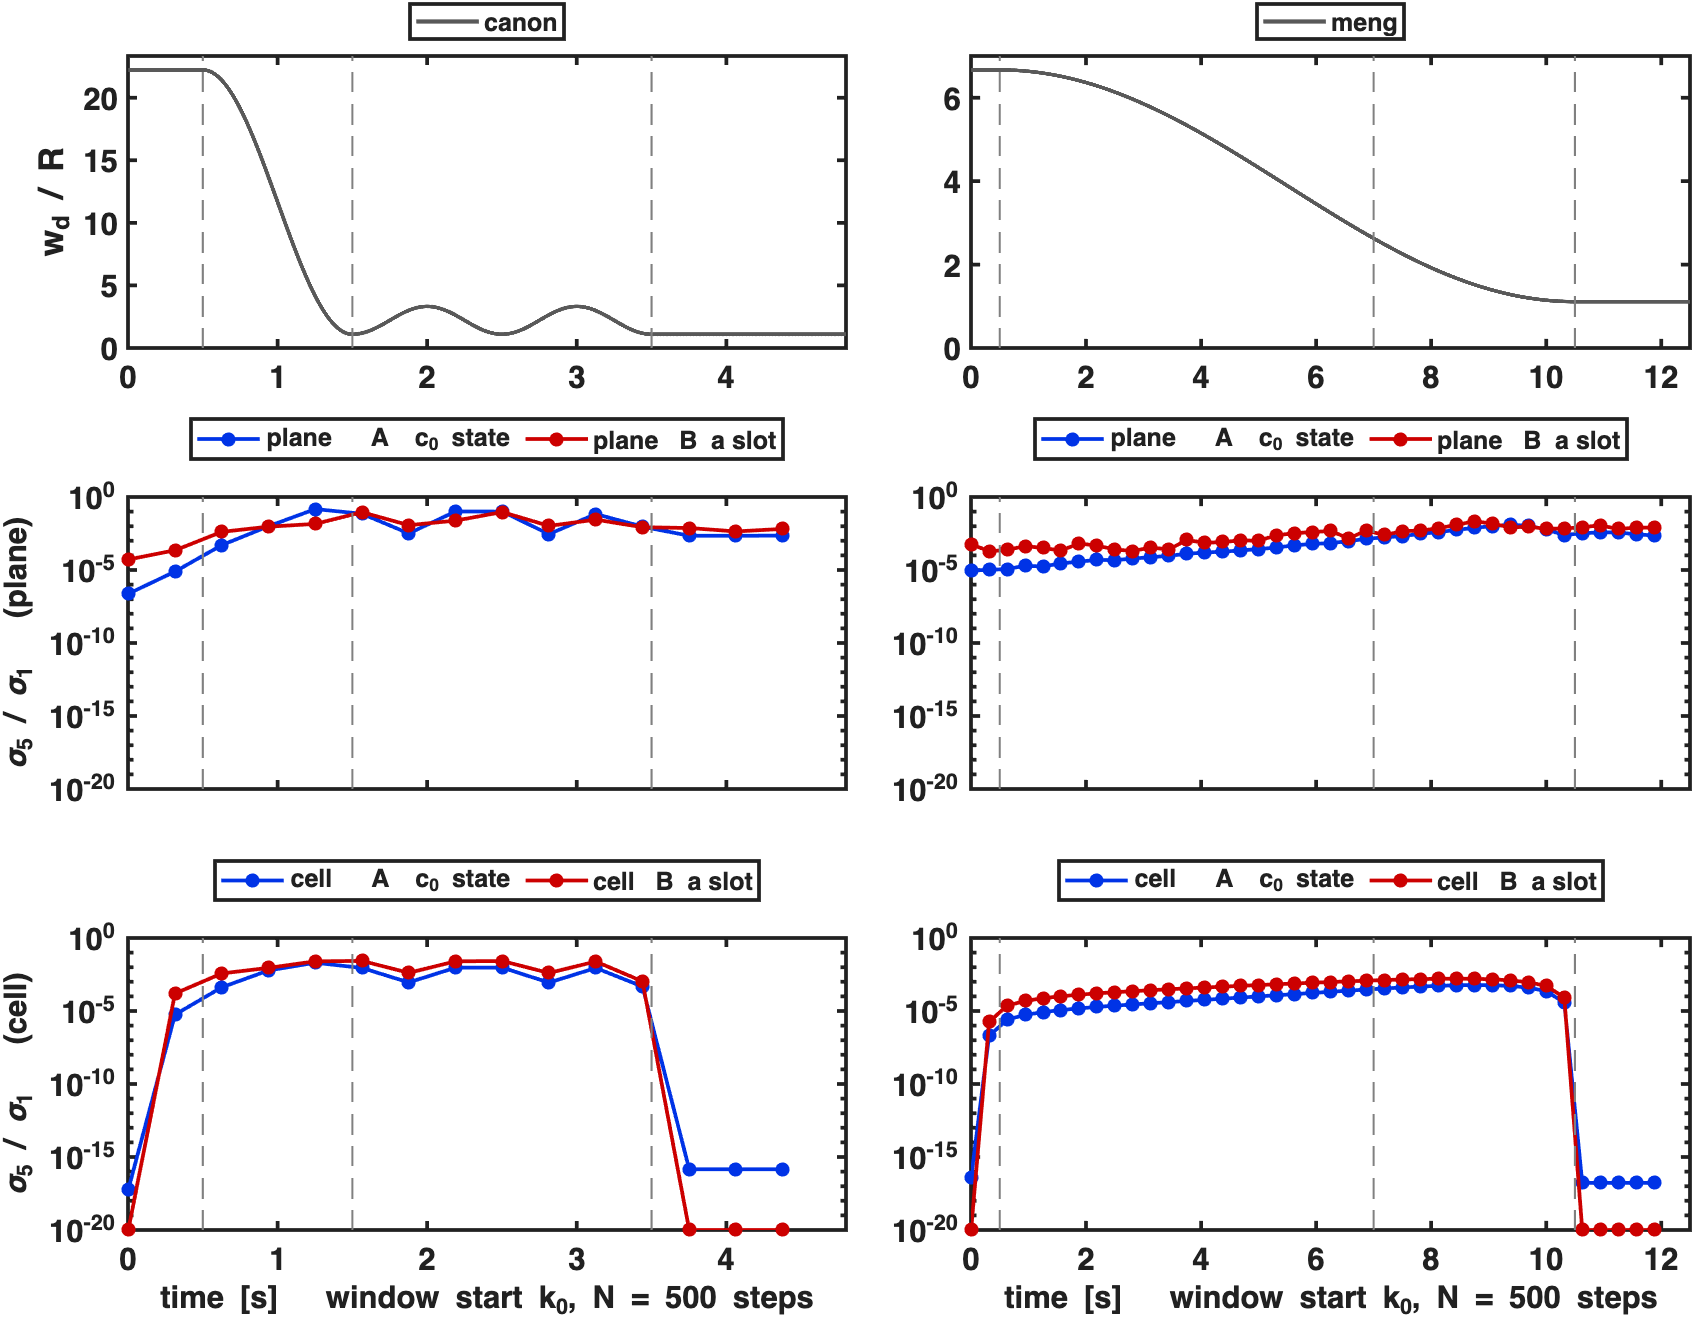
\includegraphics[width=\textwidth]{figures/obs11_ratio.png}

\begin{landscape}
\vspace*{\fill}
\noindent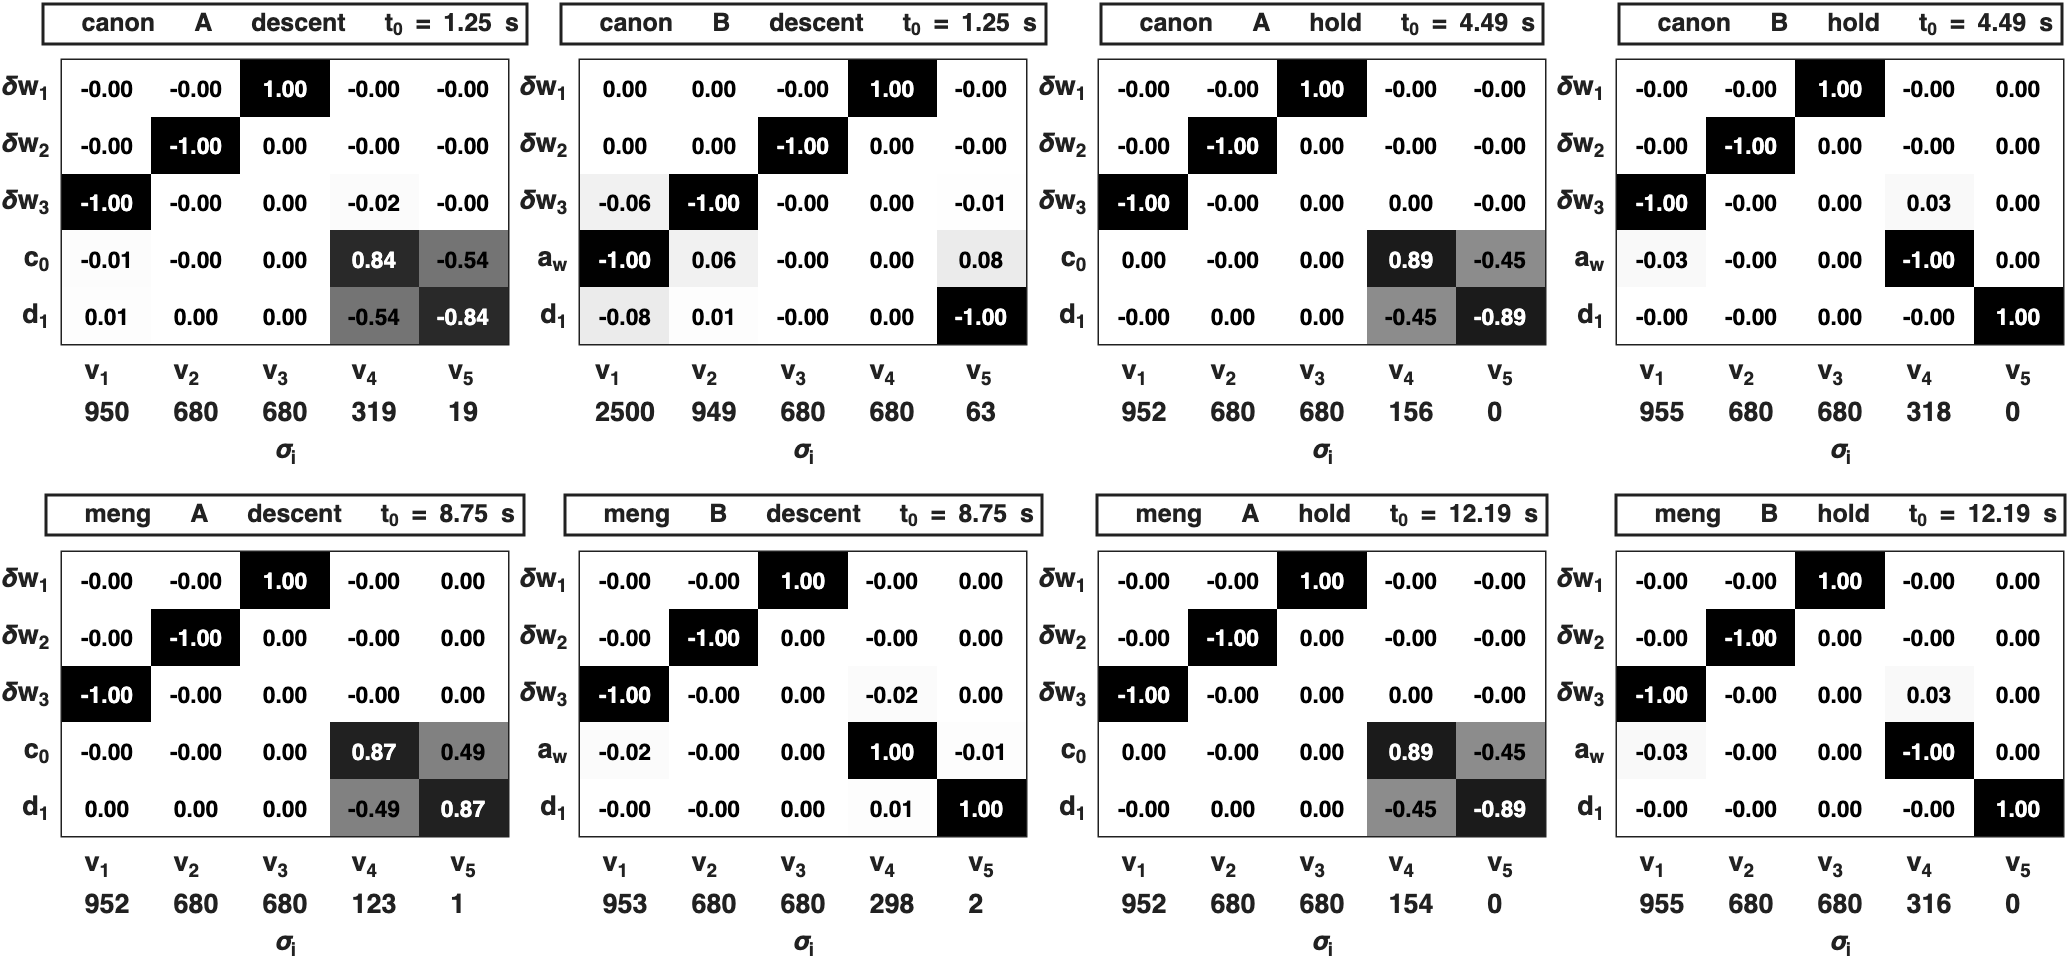
\includegraphics[width=\linewidth]{figures/obs11_sigma_V_cell.png}
\vspace*{\fill}
\end{landscape}

\begin{landscape}
\vspace*{\fill}
\noindent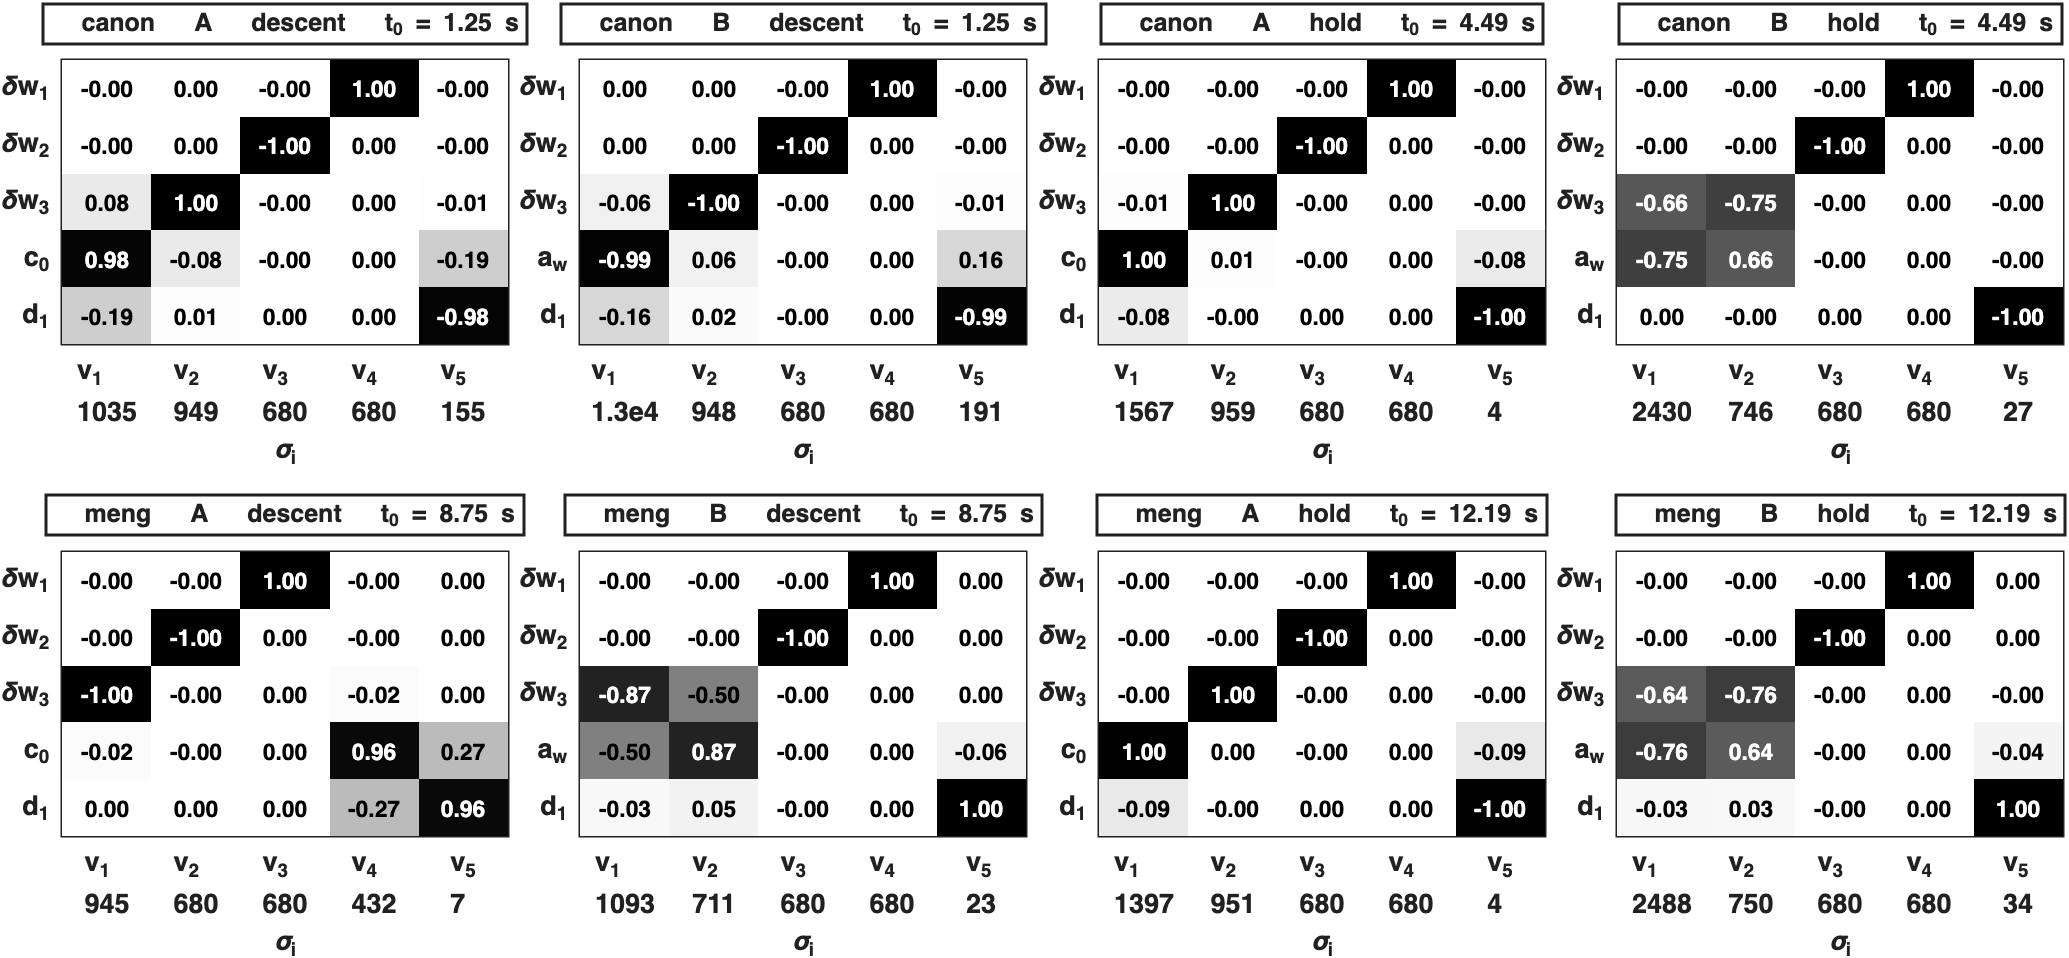
\includegraphics[width=\linewidth]{figures/obs11_sigma_V_plane.png}
\vspace*{\fill}
\end{landscape}

\clearpage
\noindent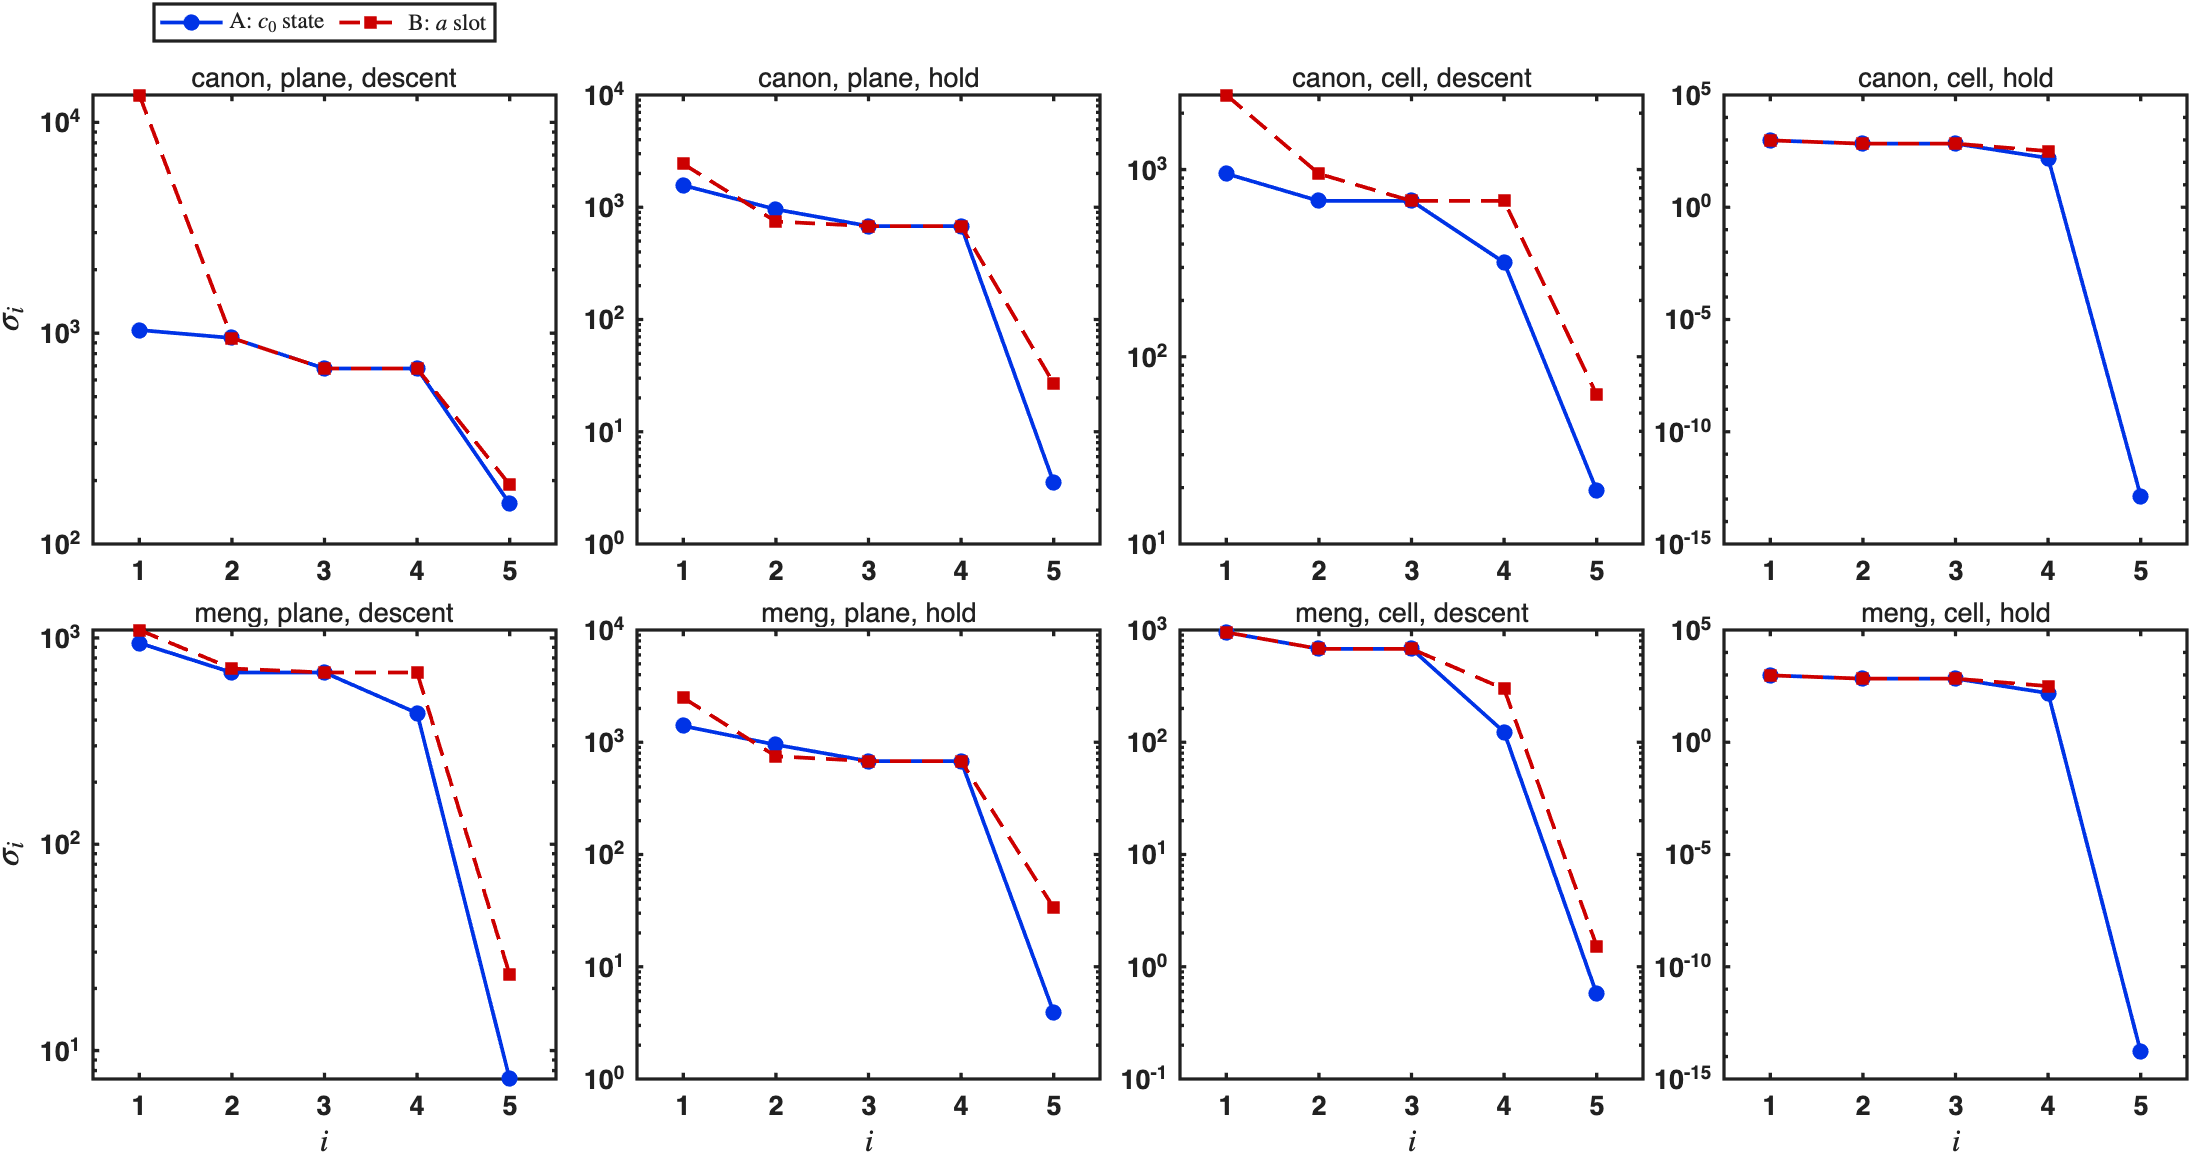
\includegraphics[width=\textwidth]{figures/obs11_sigma.png}

\begin{landscape}
\vspace*{\fill}
\noindent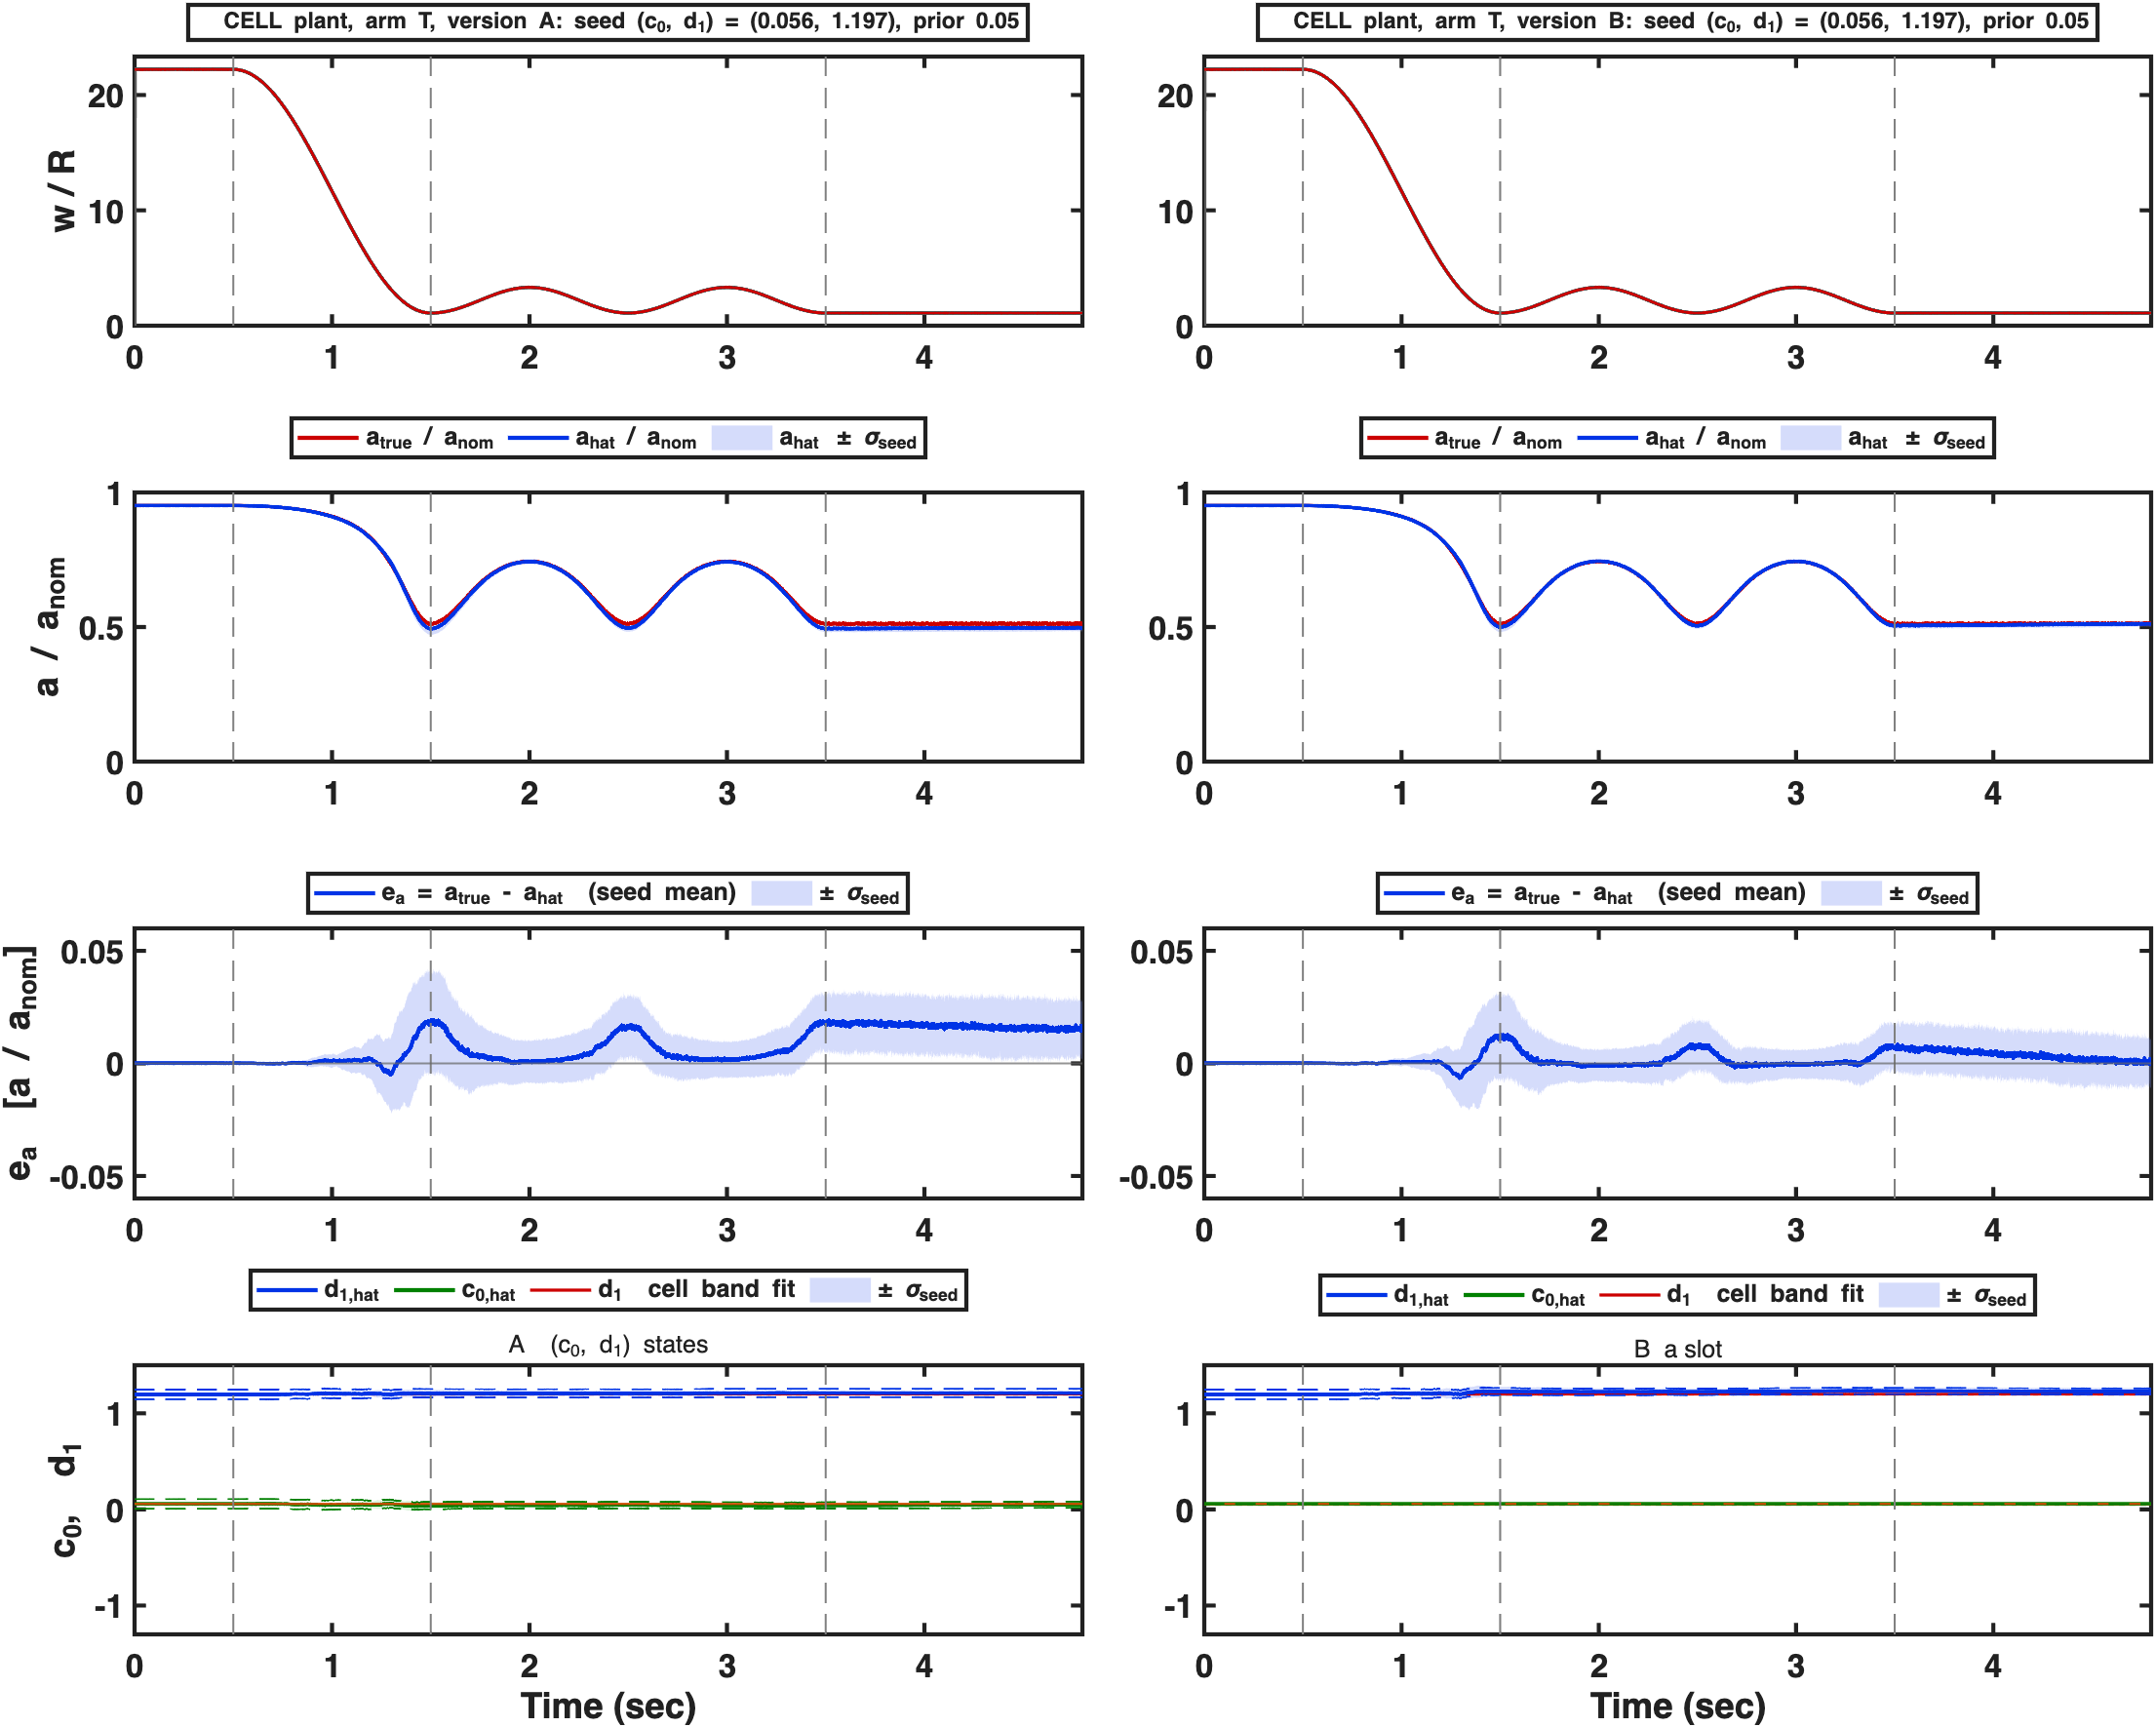
\includegraphics[height=0.95\textheight]{figures/ladder11_cell_T.png}
\vspace*{\fill}
\end{landscape}

\begin{landscape}
\vspace*{\fill}
\noindent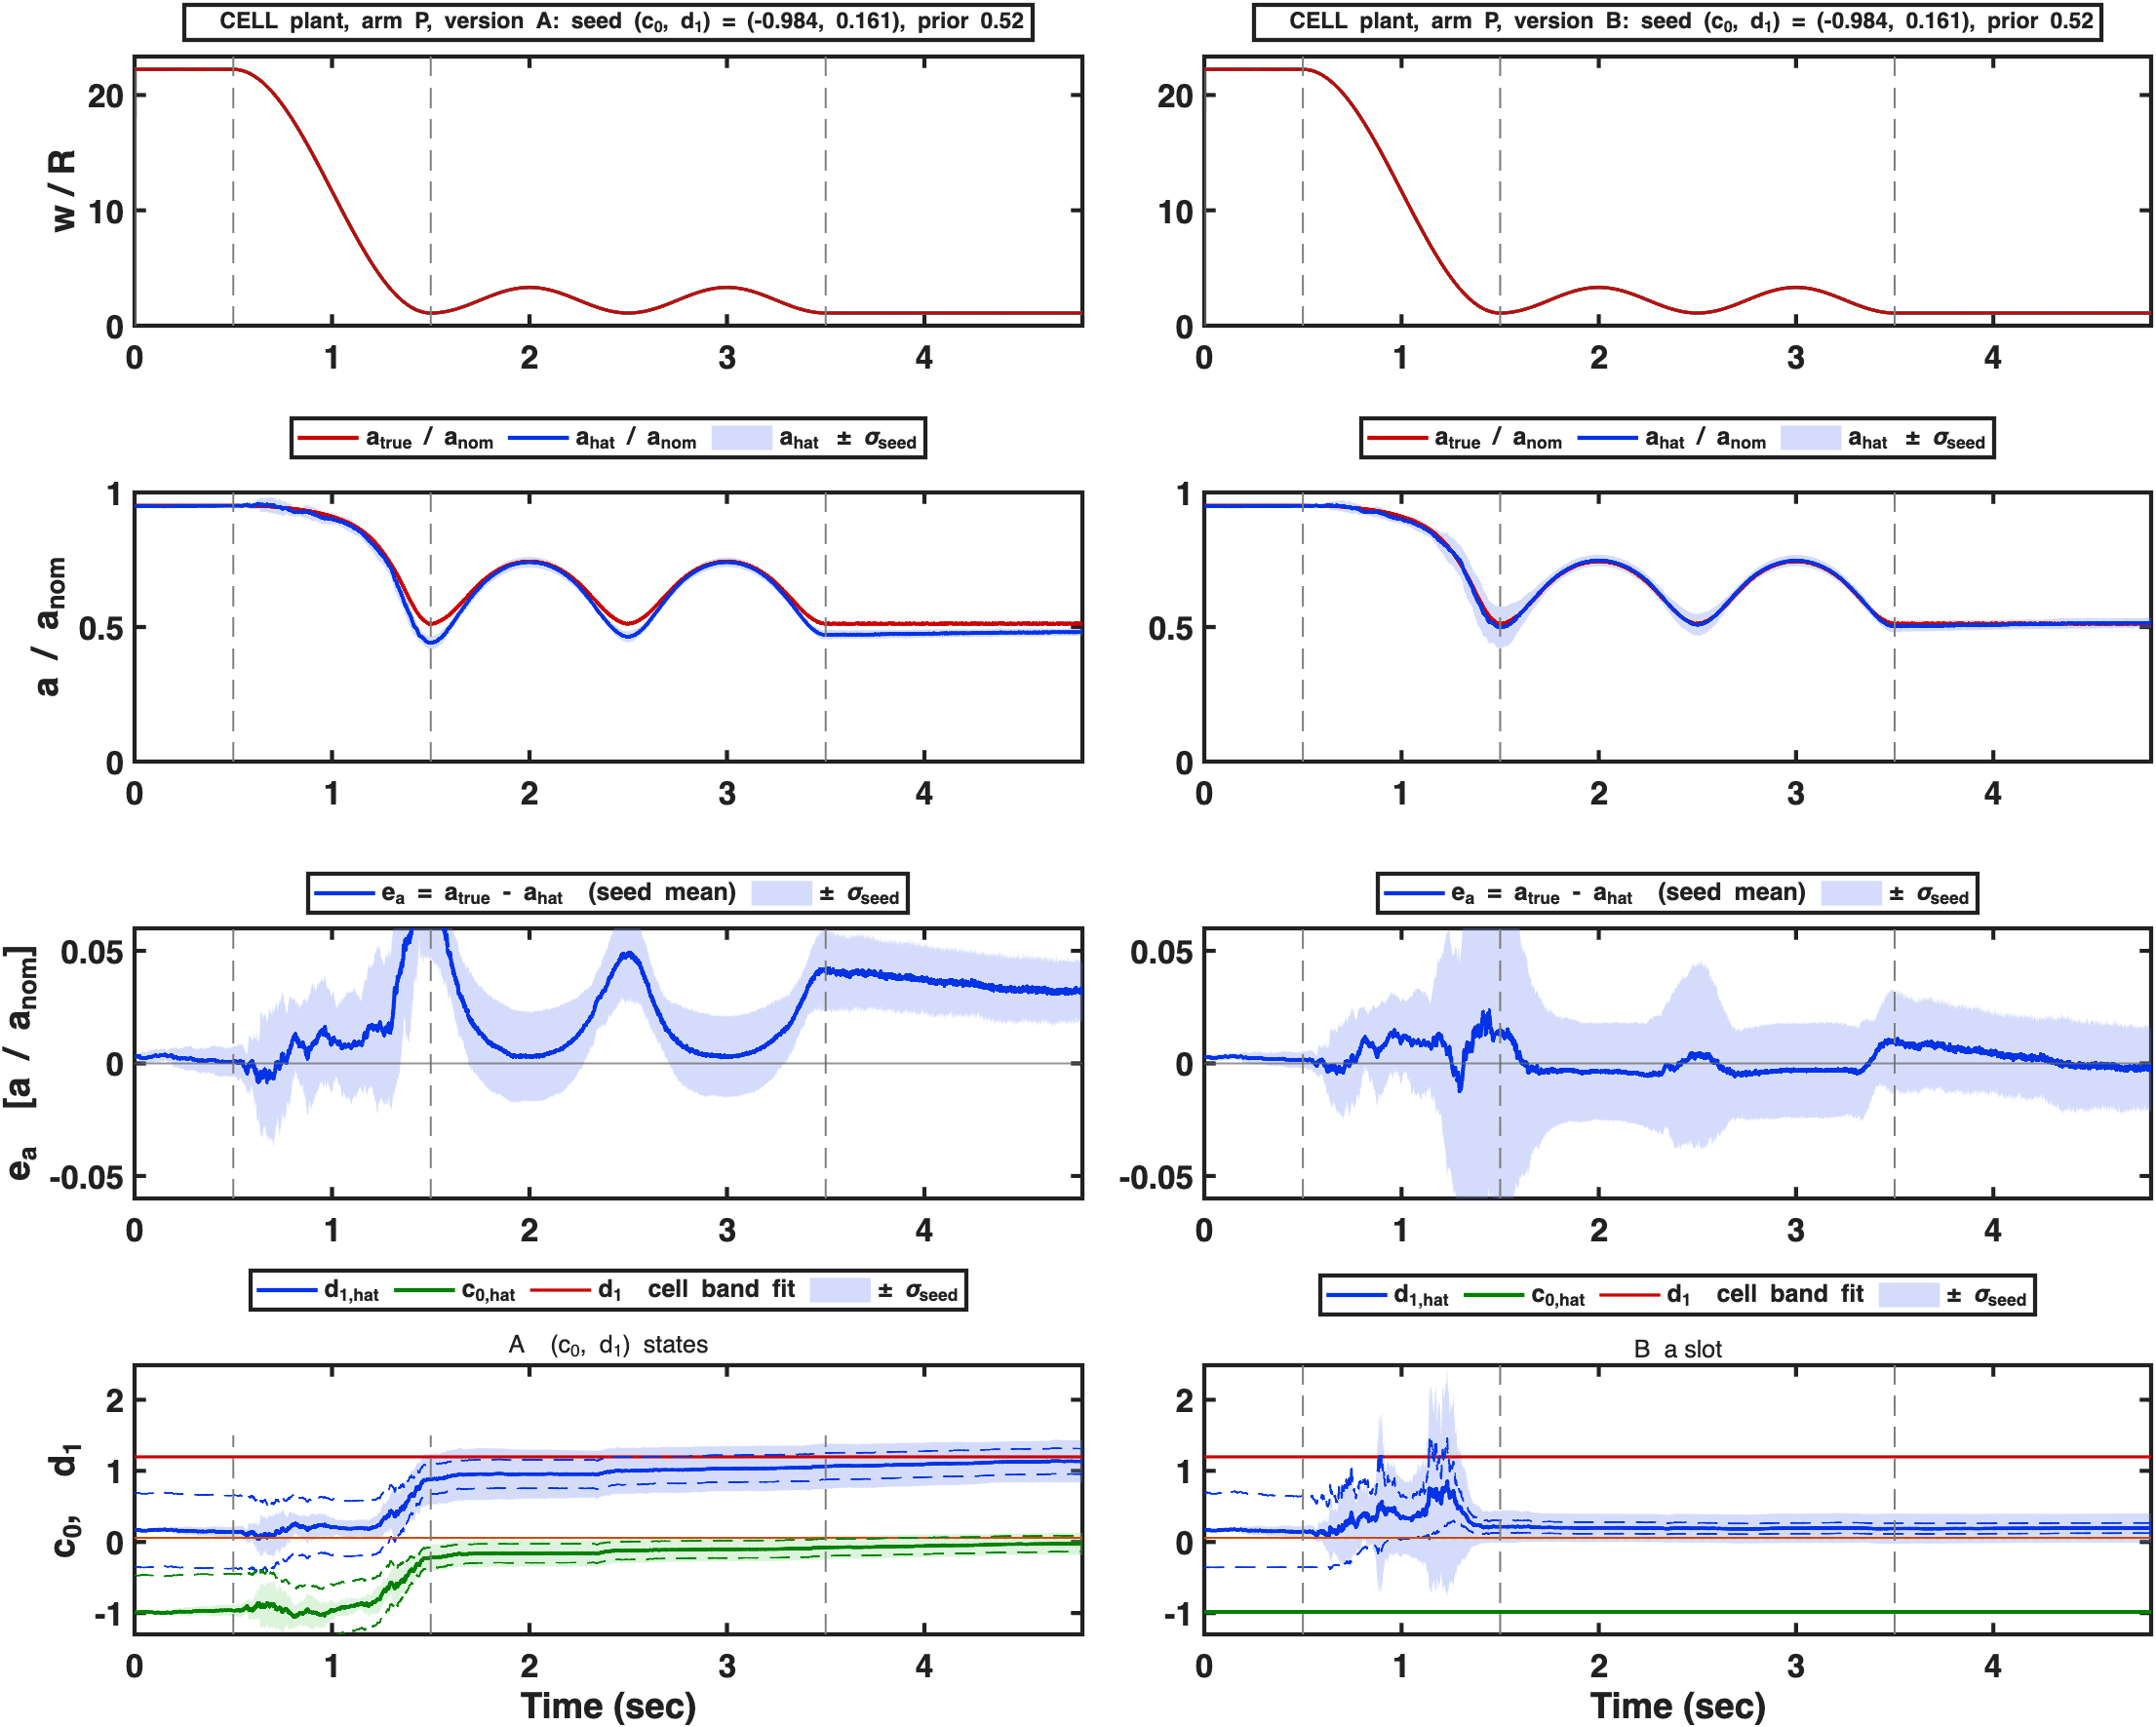
\includegraphics[height=0.95\textheight]{figures/ladder11_cell_P.png}
\vspace*{\fill}
\end{landscape}

\begin{landscape}
\vspace*{\fill}
\noindent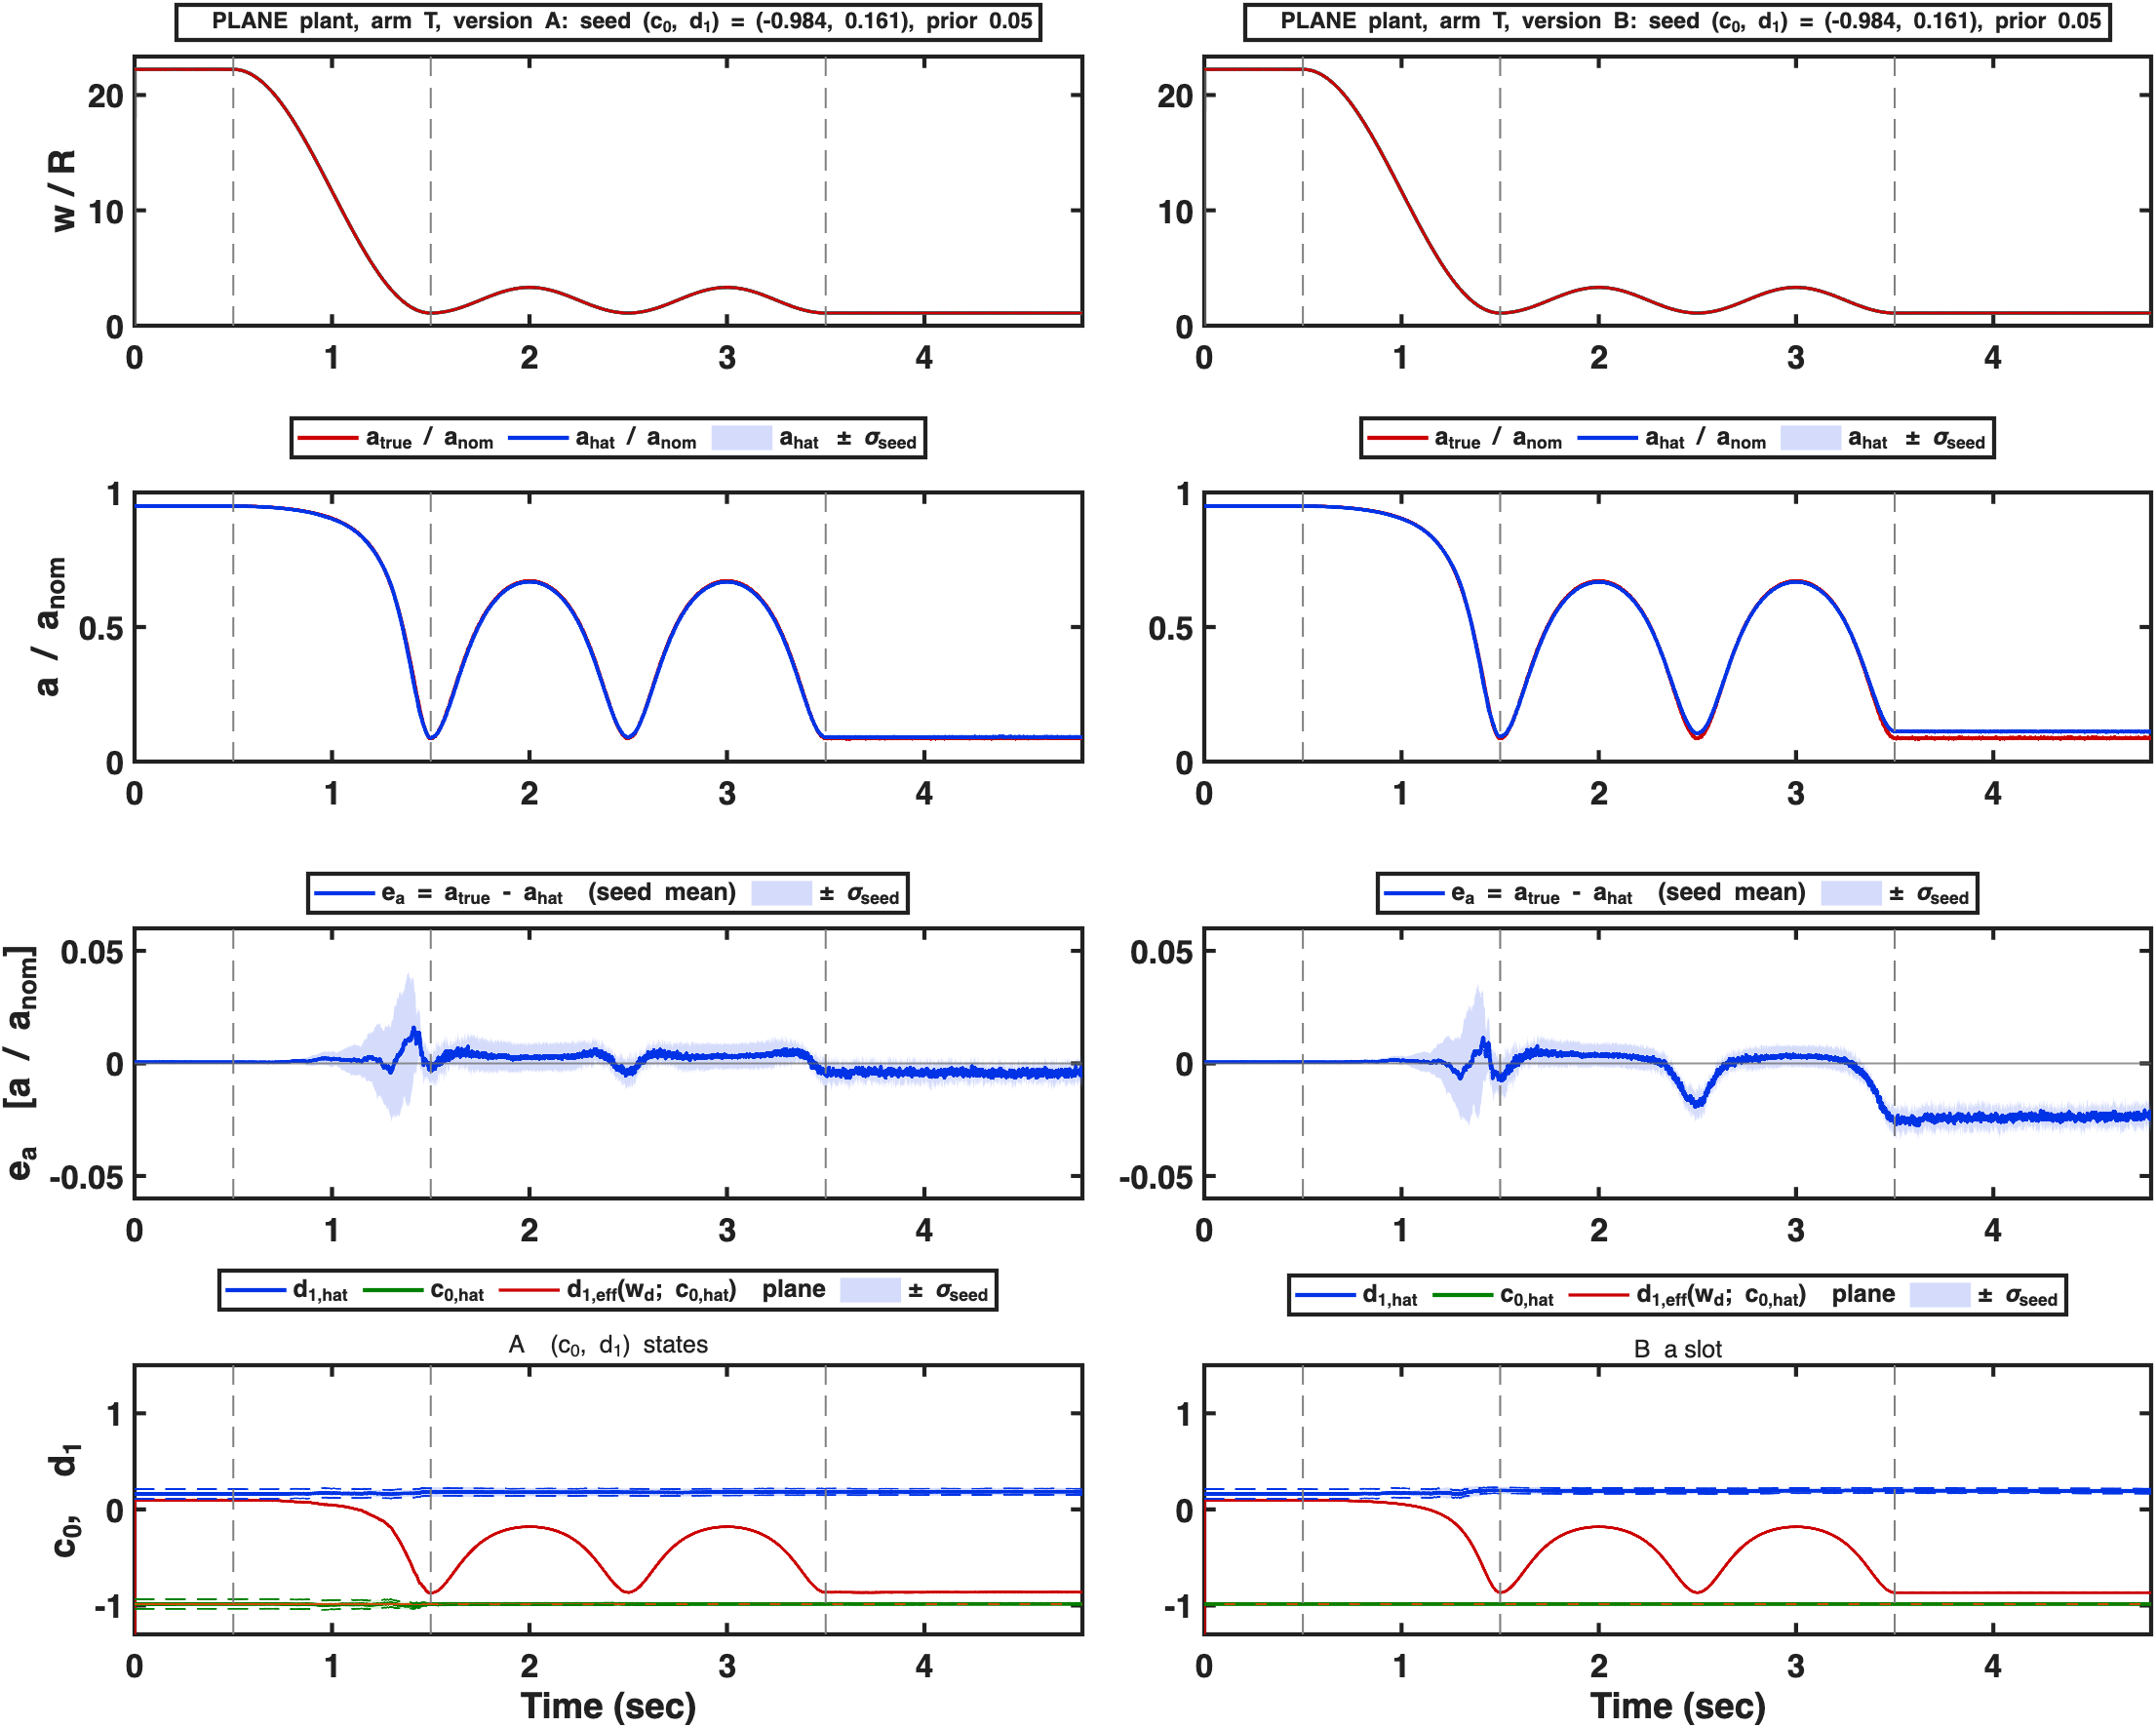
\includegraphics[height=0.95\textheight]{figures/ladder11_plane_T.png}
\vspace*{\fill}
\end{landscape}

\begin{landscape}
\vspace*{\fill}
\noindent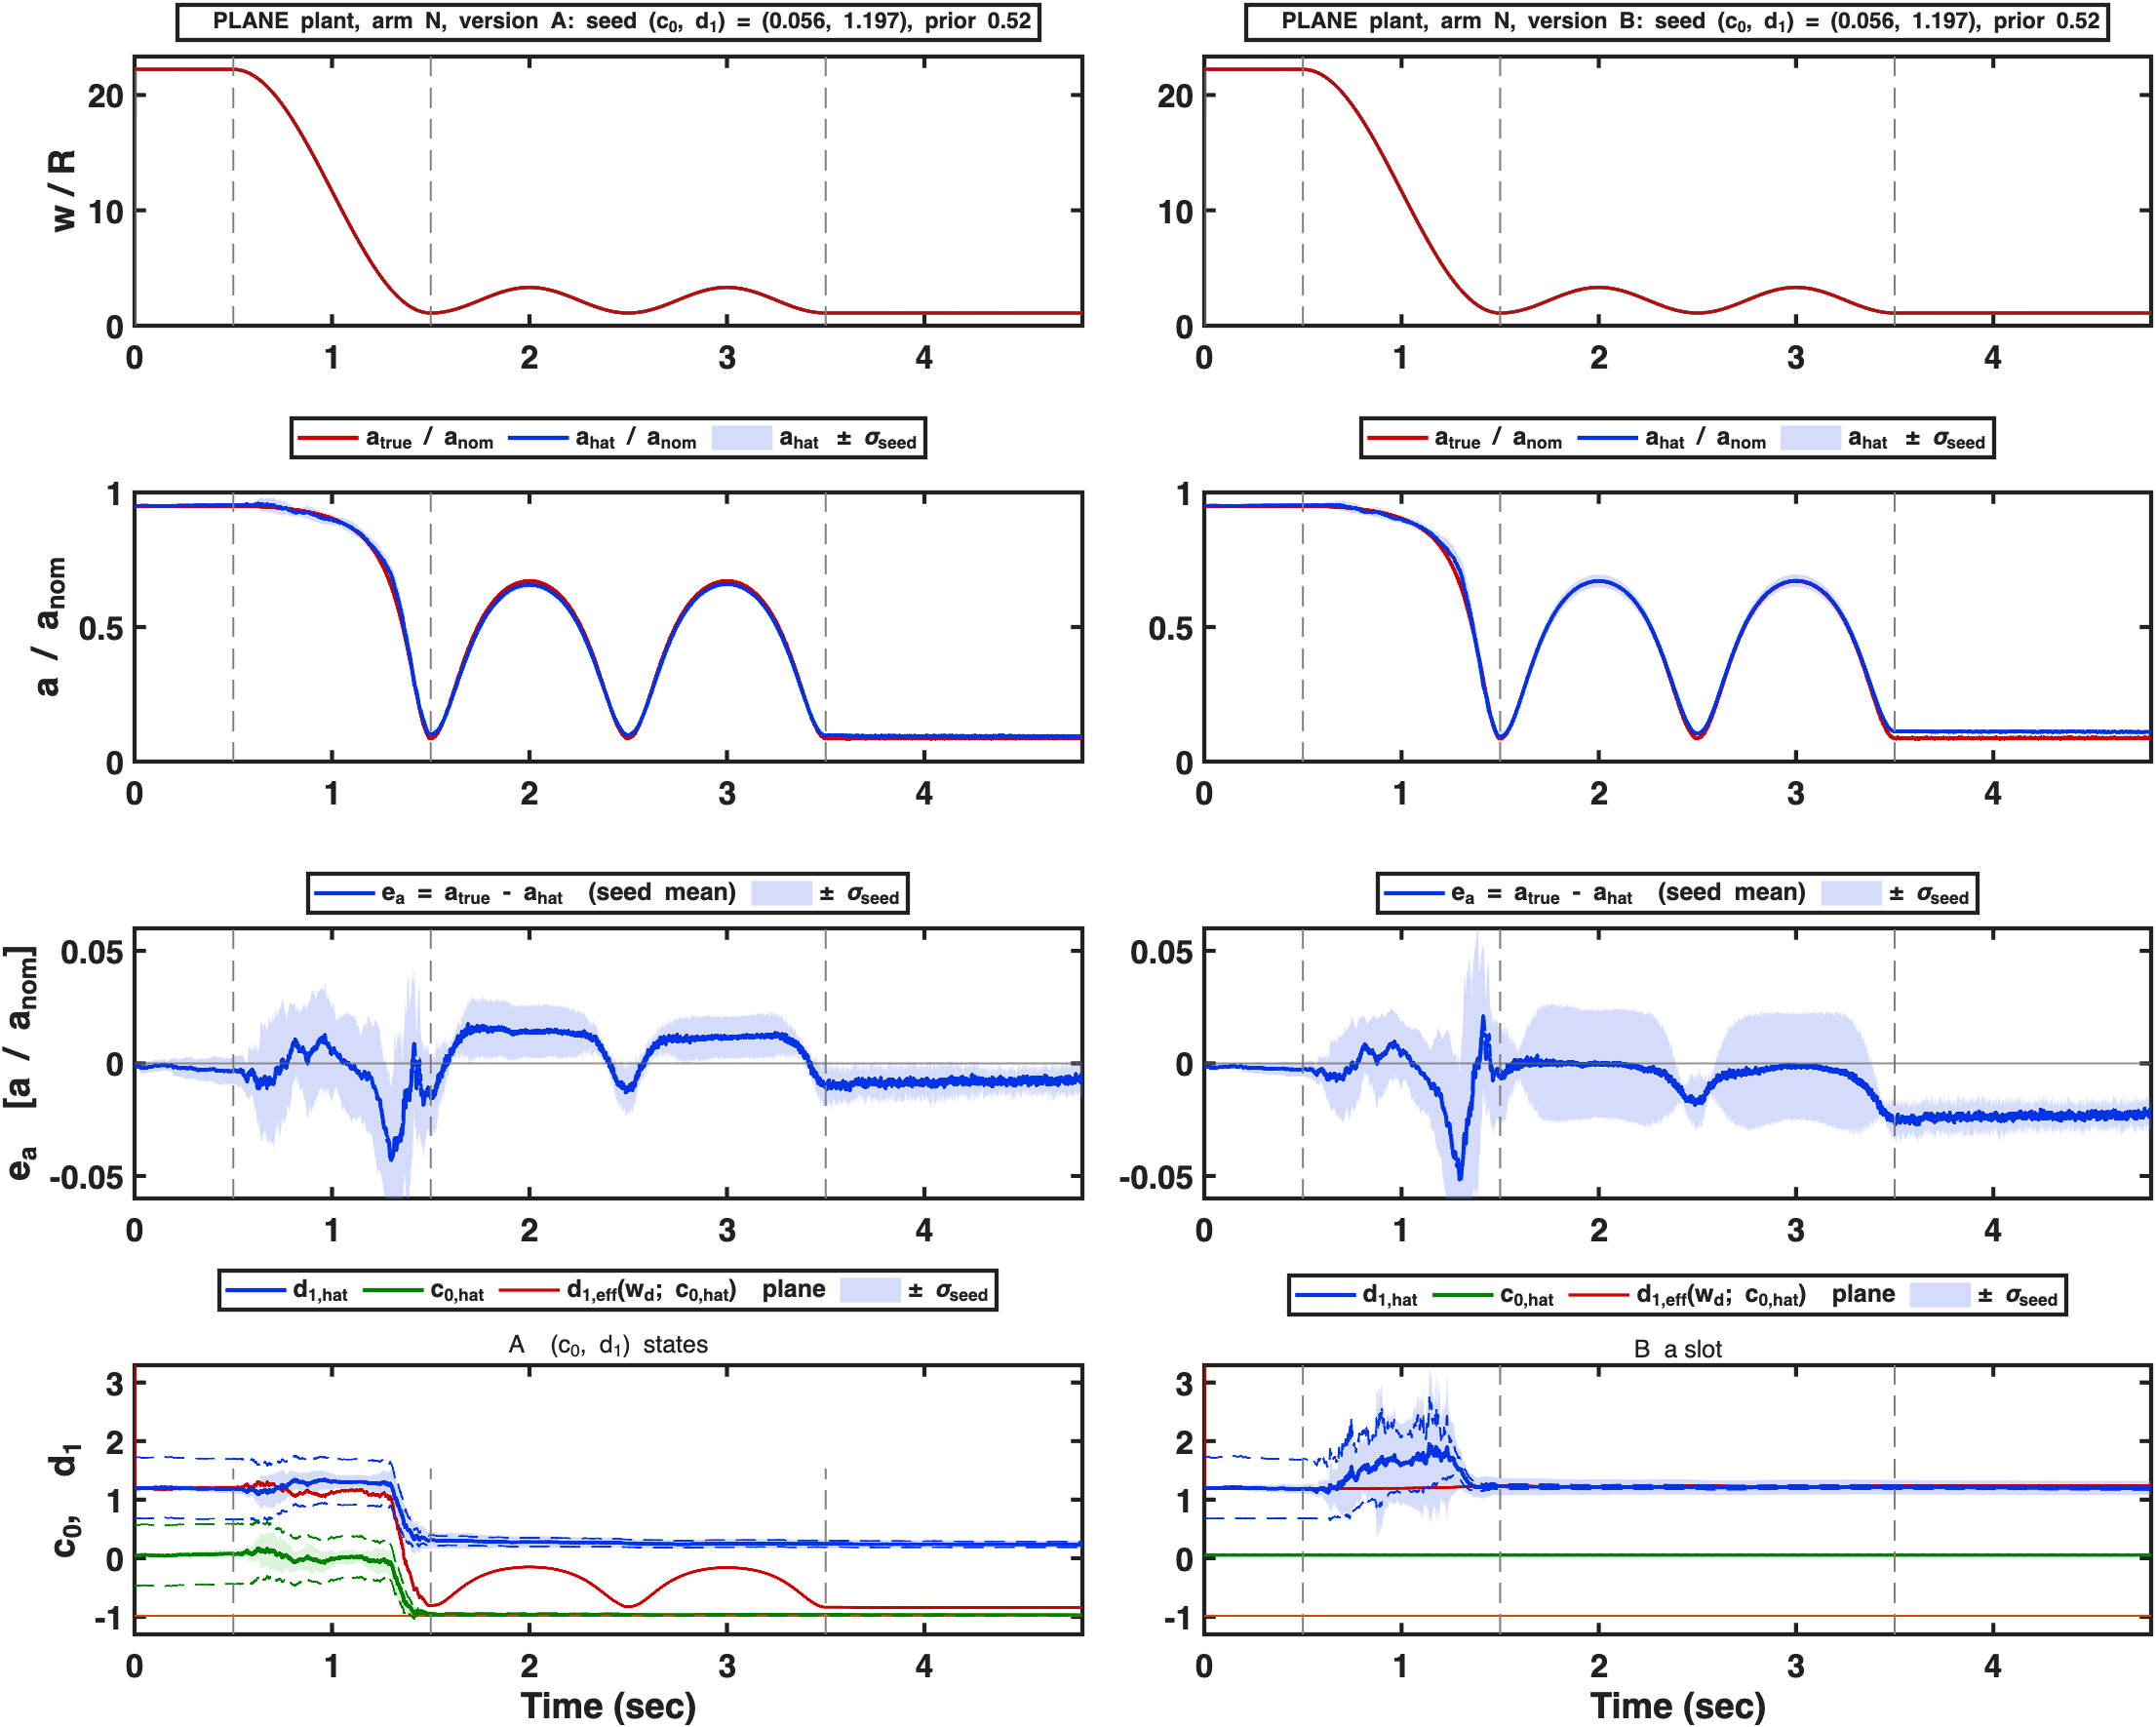
\includegraphics[height=0.95\textheight]{figures/ladder11_plane_N.png}
\vspace*{\fill}
\end{landscape}

\begin{landscape}
\vspace*{\fill}
\noindent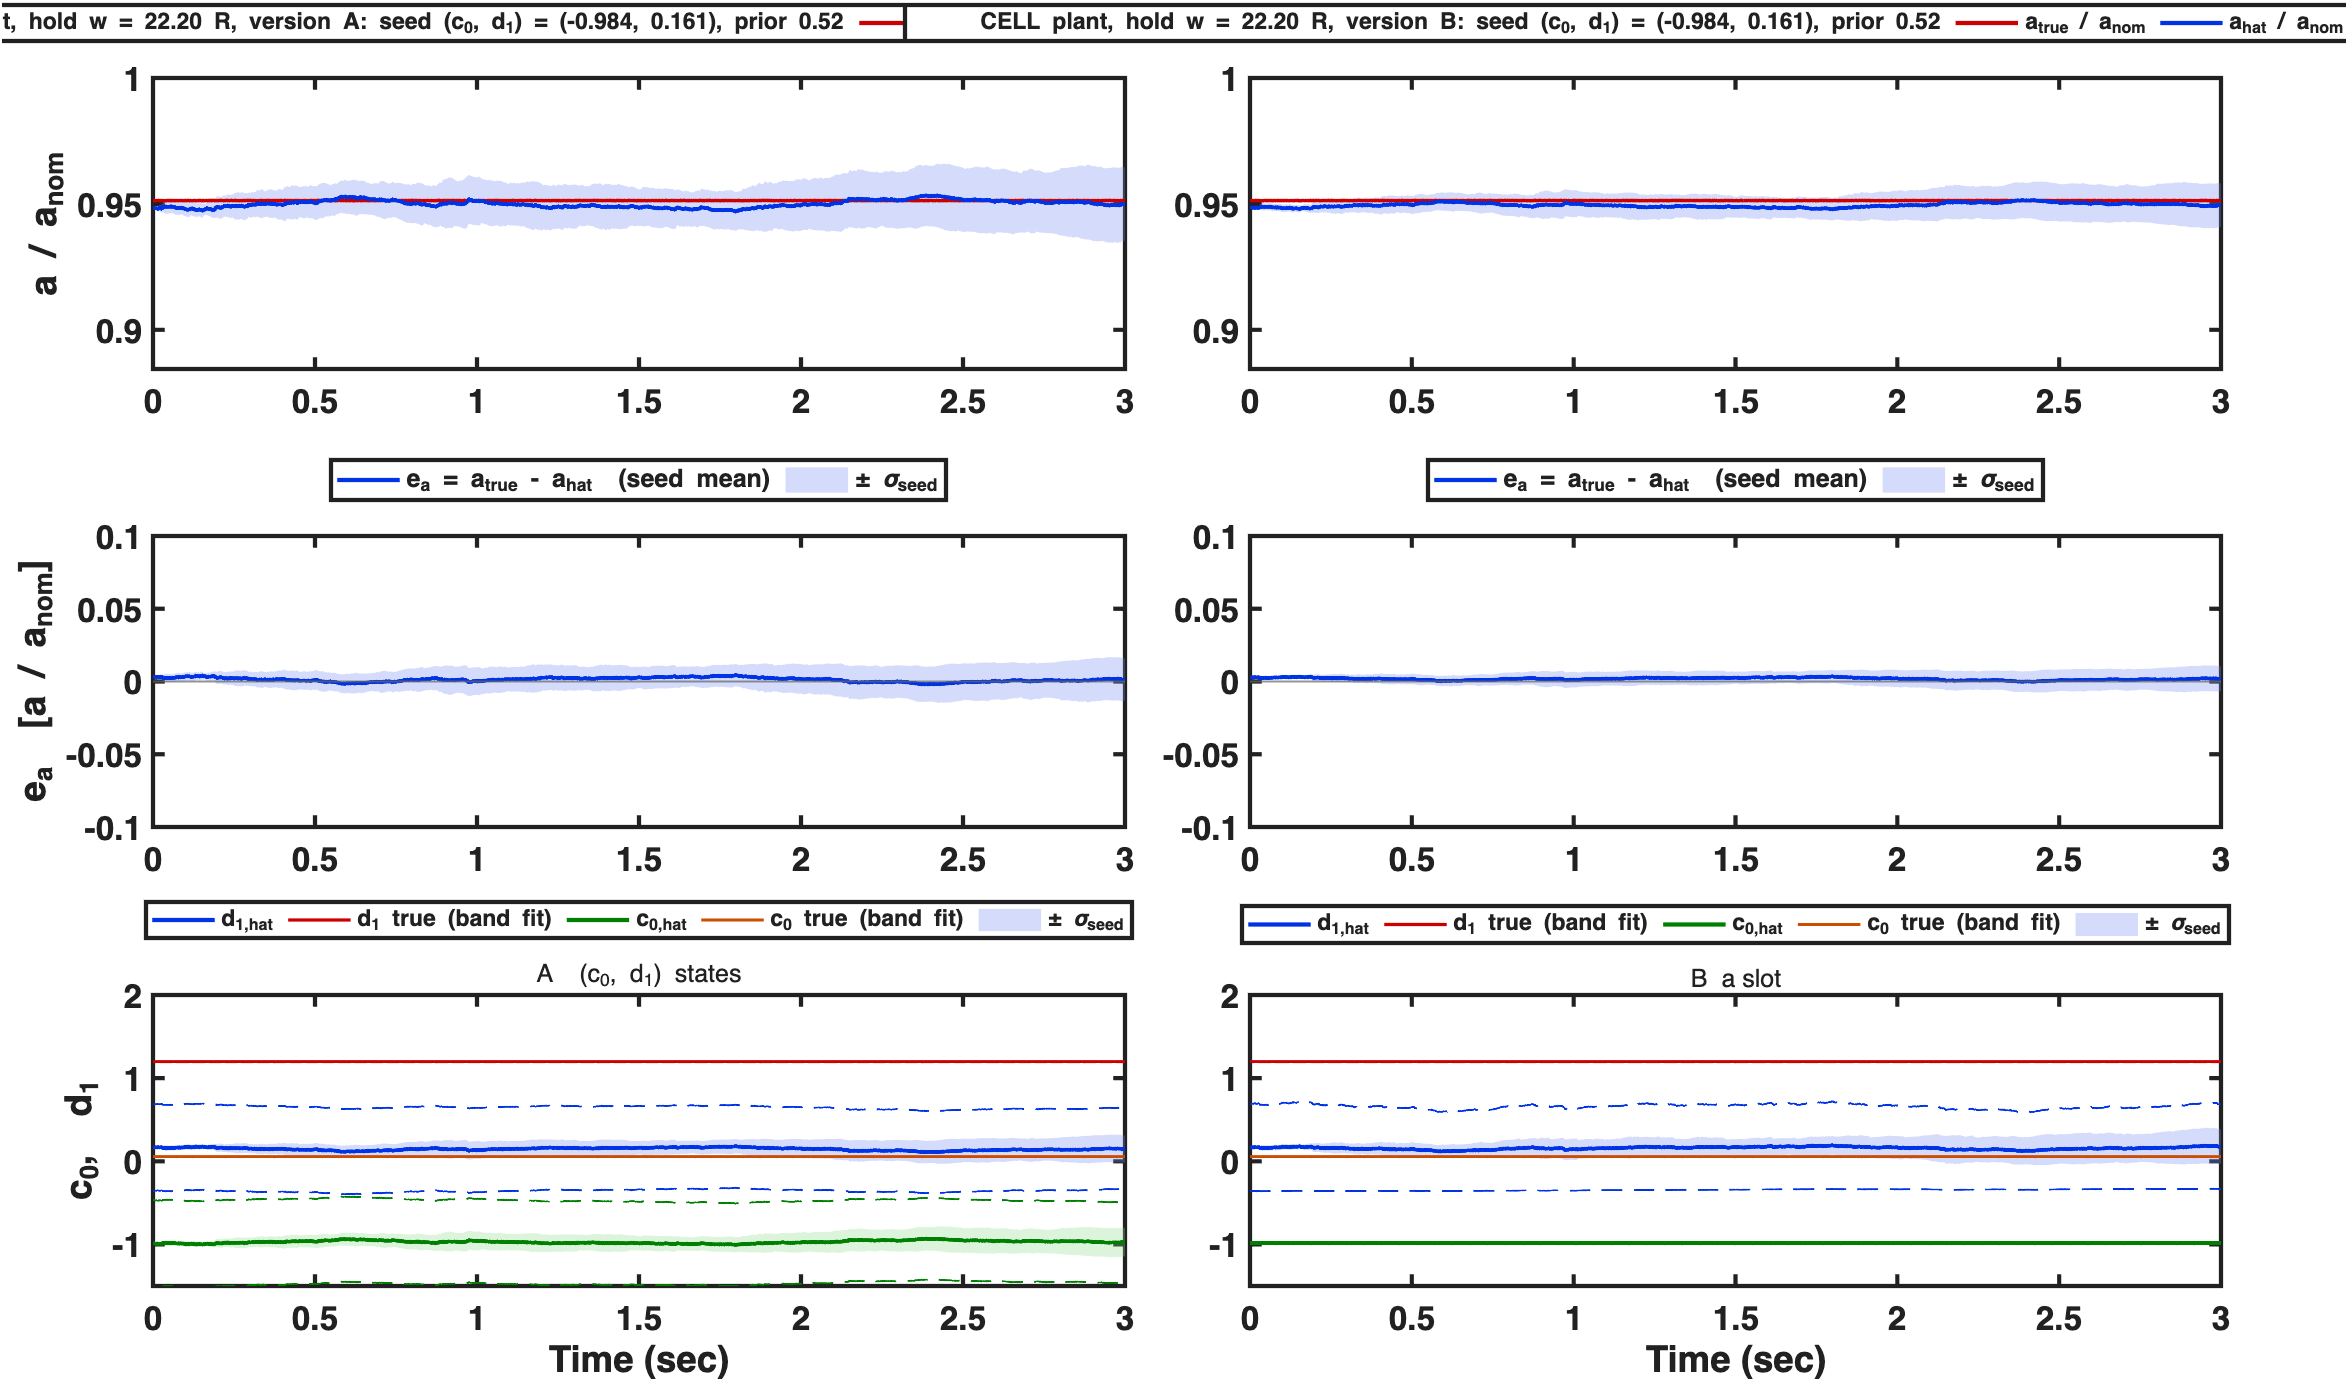
\includegraphics[width=\linewidth]{figures/fixed11_cell_h22p20.png}
\vspace*{\fill}
\end{landscape}

\begin{landscape}
\vspace*{\fill}
\noindent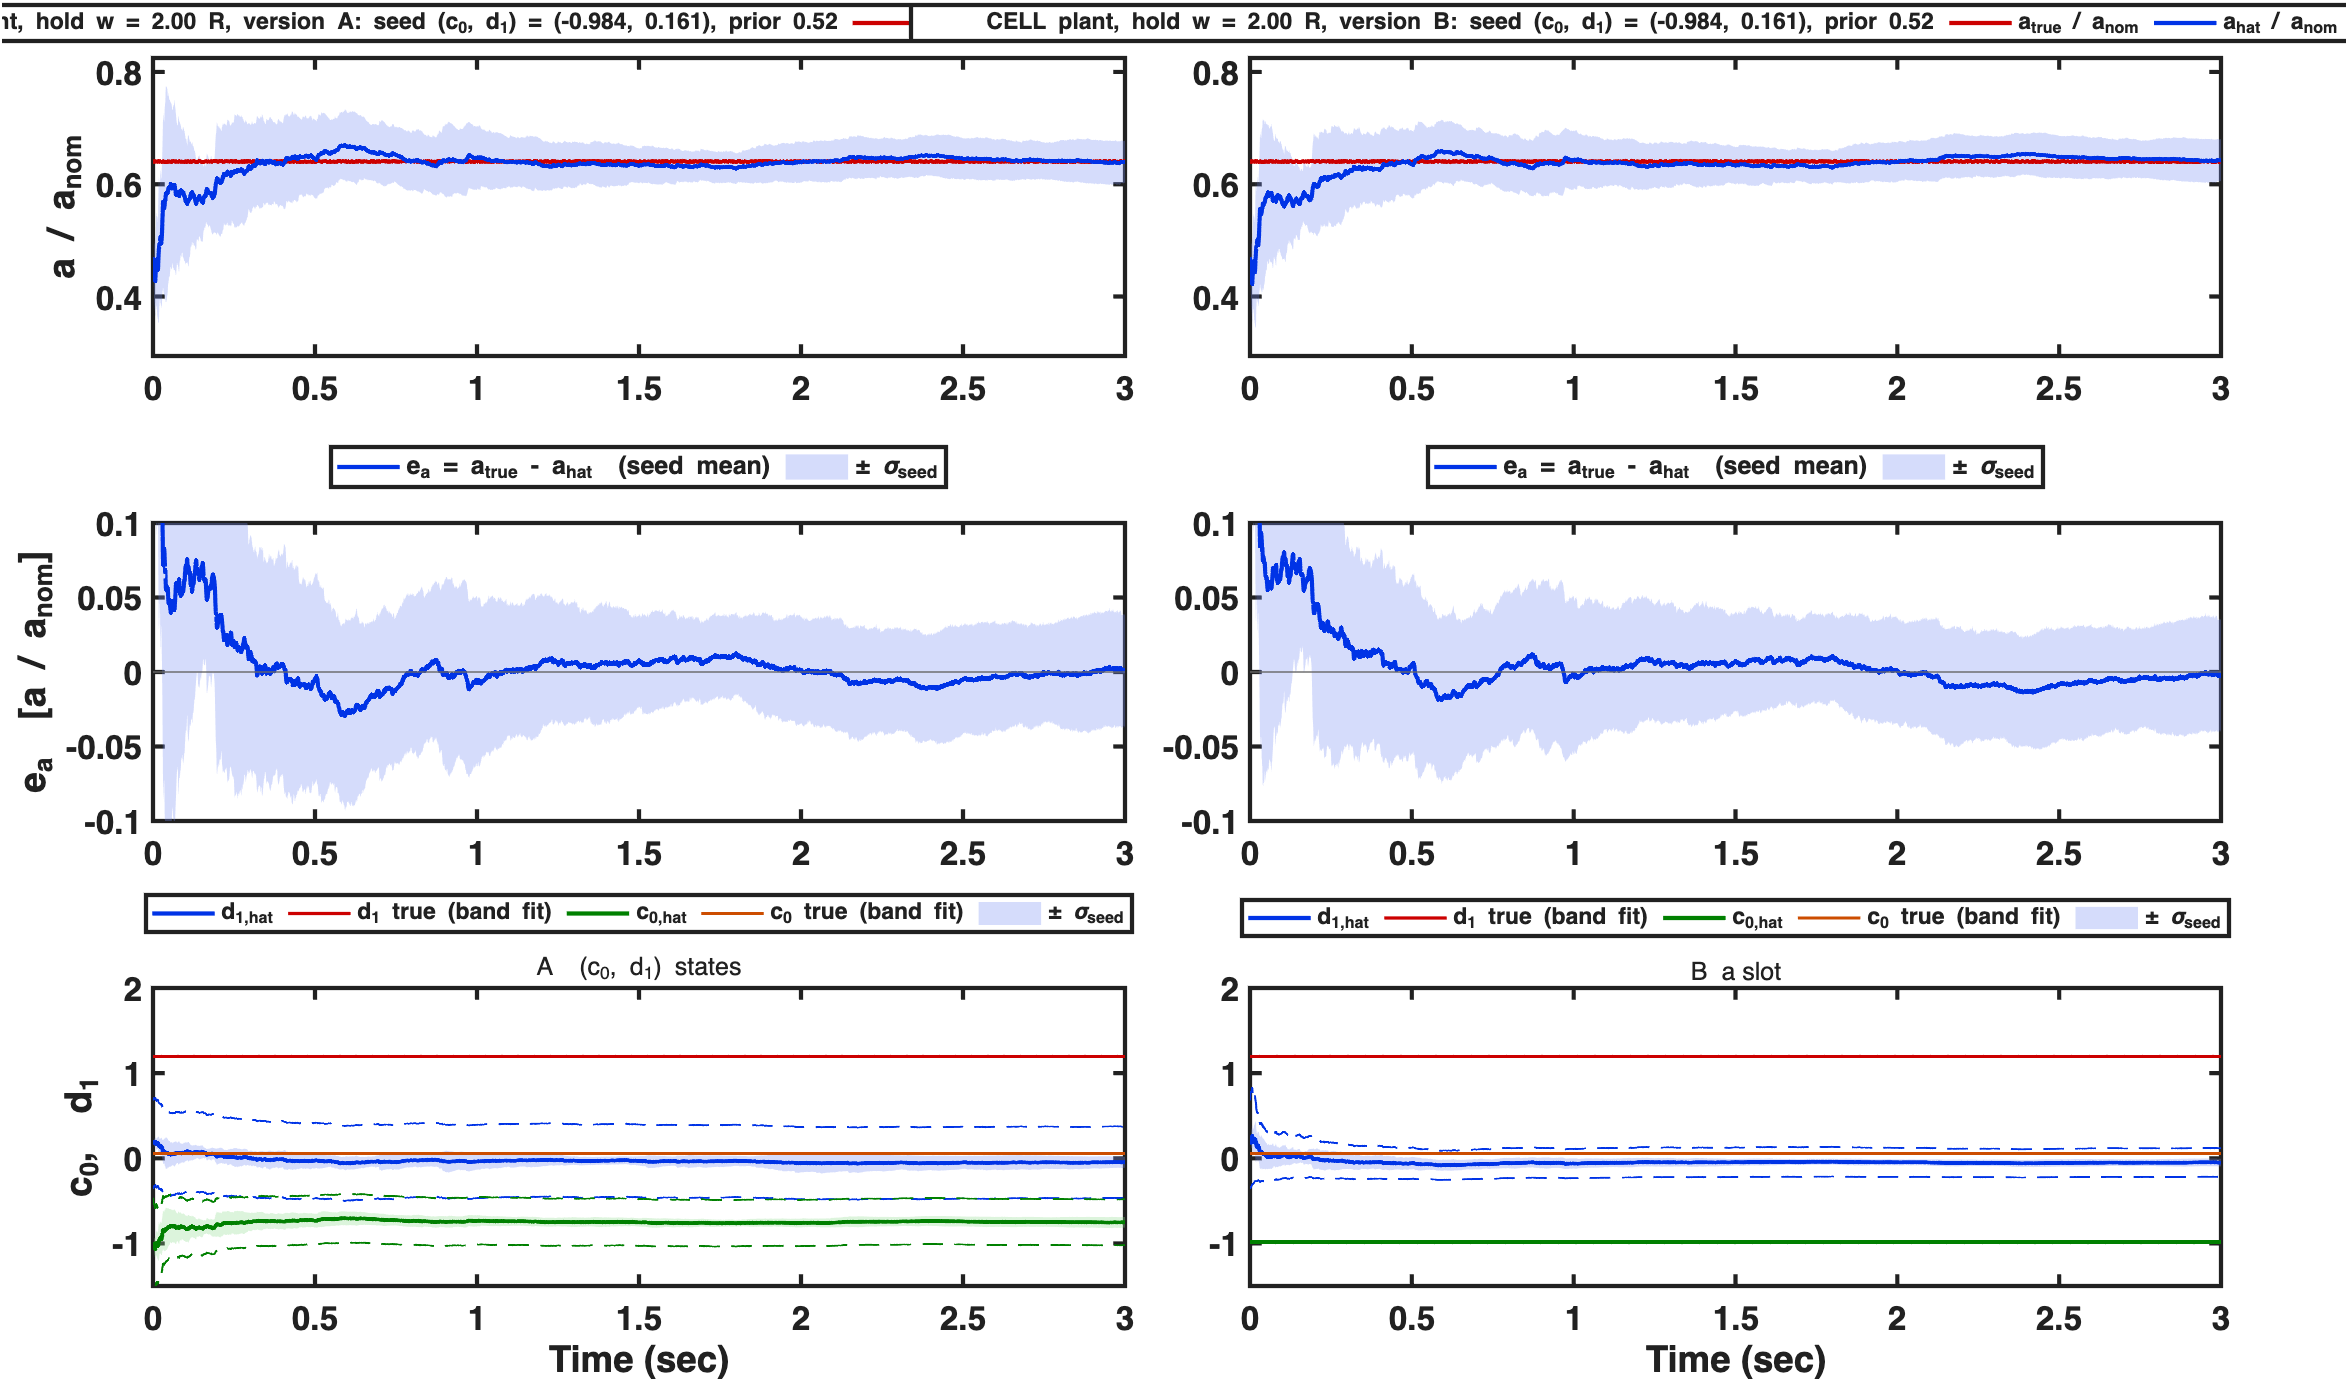
\includegraphics[width=\linewidth]{figures/fixed11_cell_h2p00.png}
\vspace*{\fill}
\end{landscape}

\begin{landscape}
\vspace*{\fill}
\noindent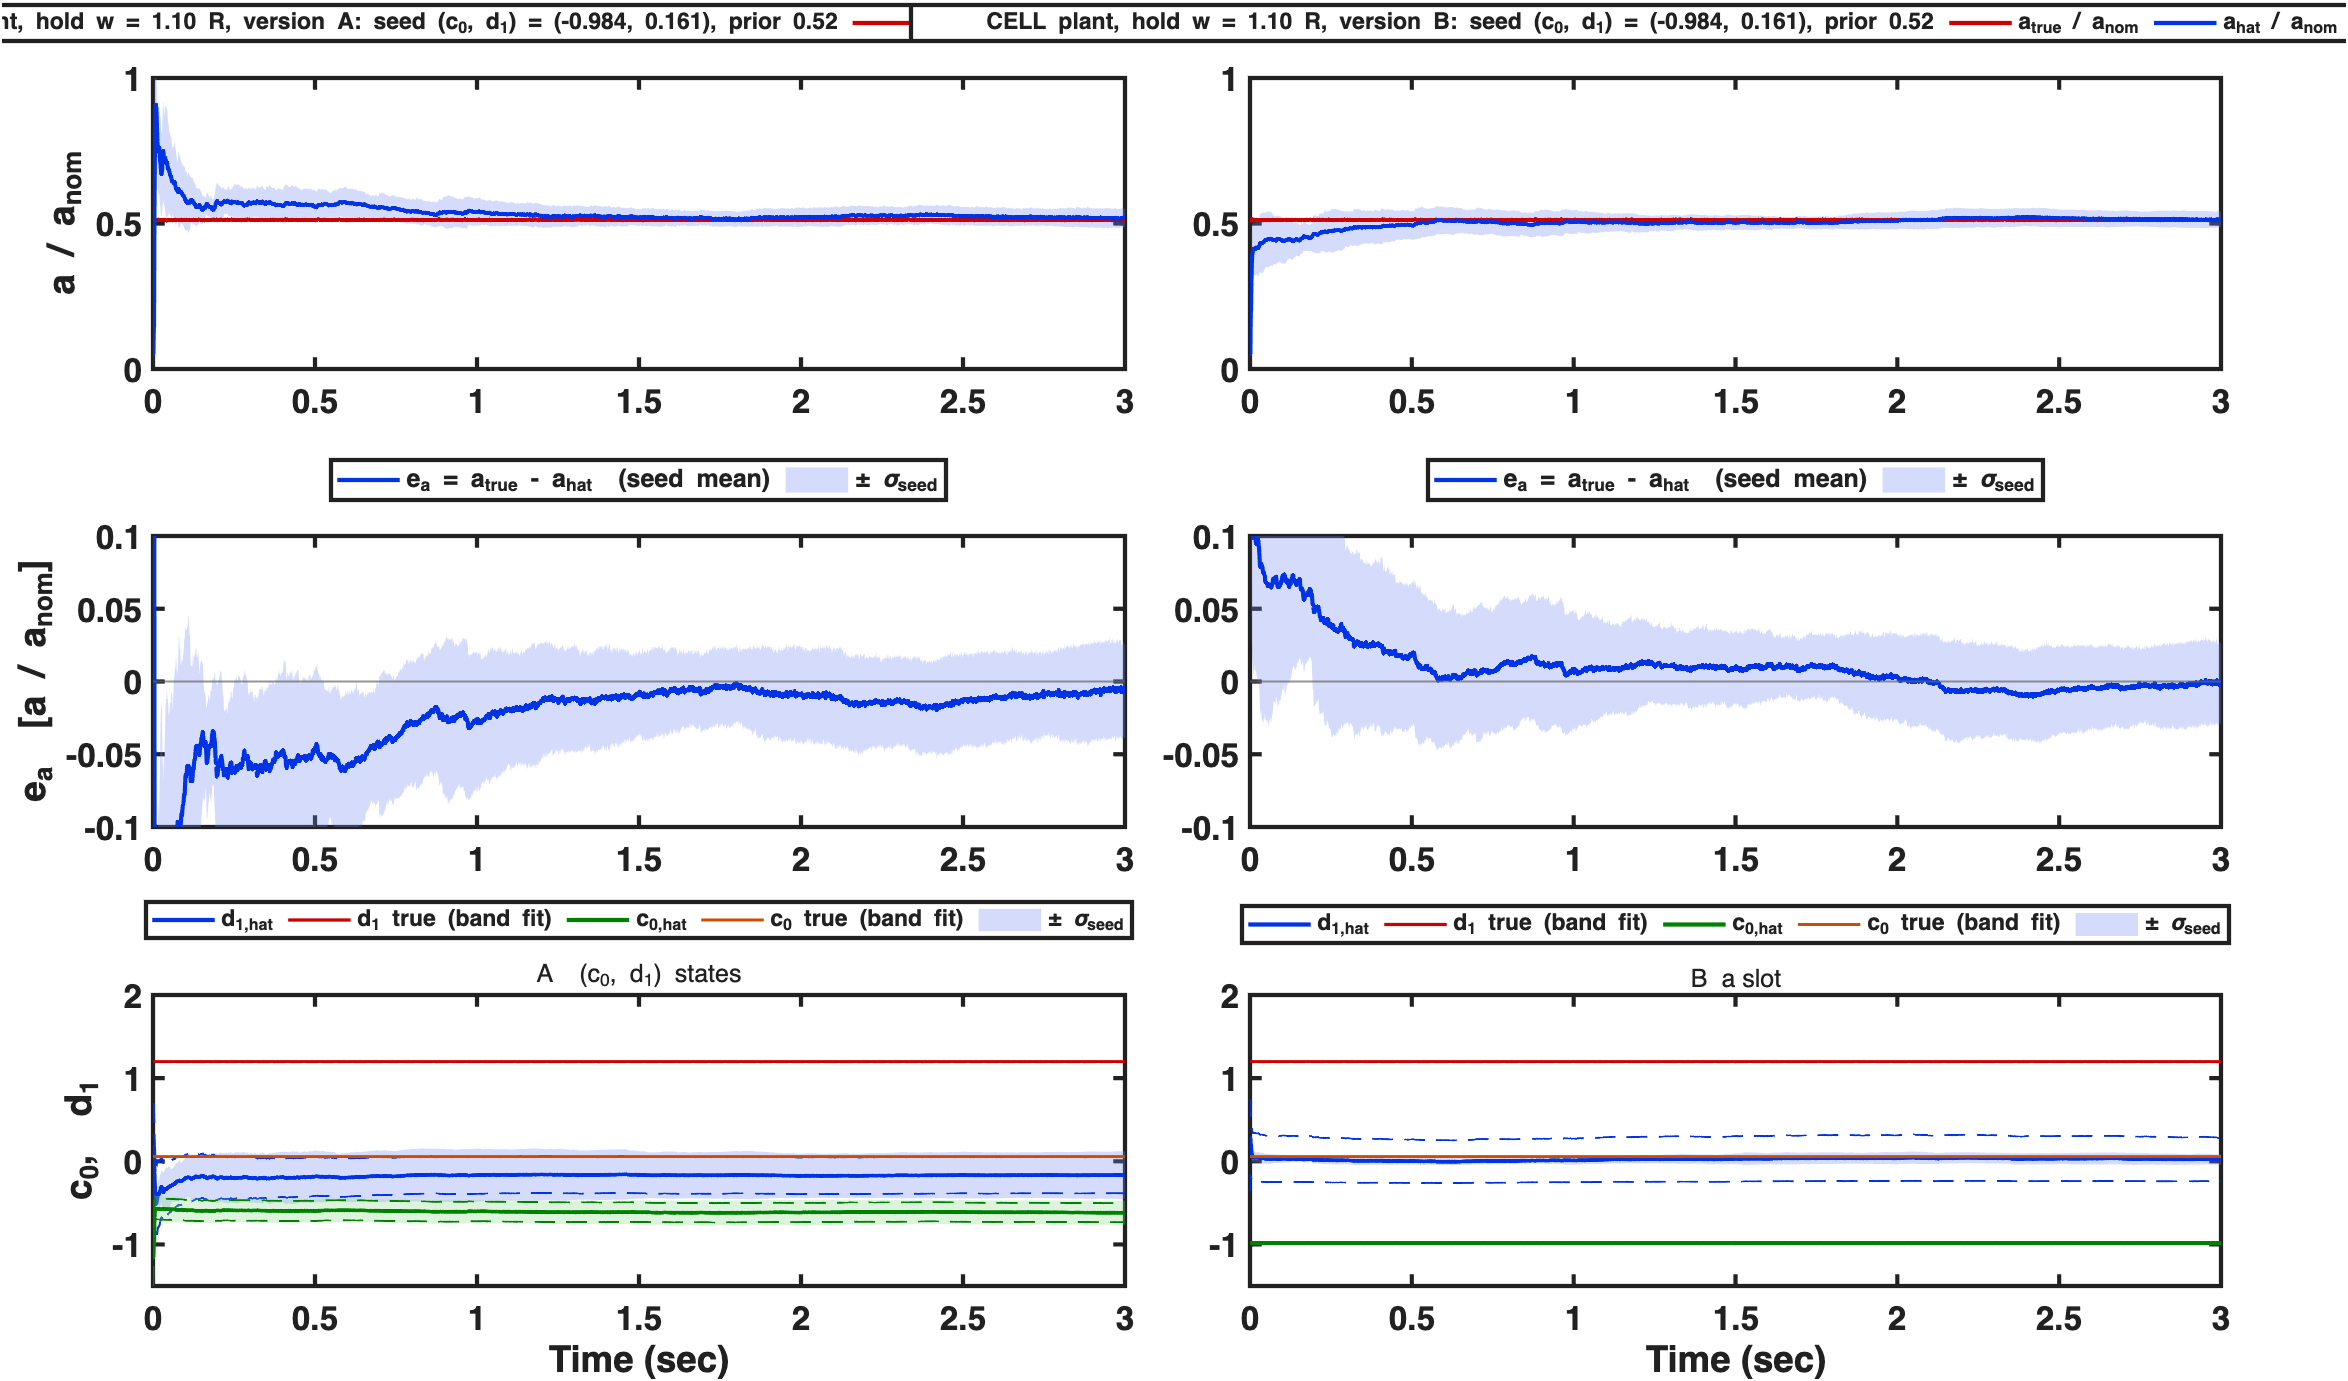
\includegraphics[width=\linewidth]{figures/fixed11_cell_h1p10.png}
\vspace*{\fill}
\end{landscape}

\clearpage
\noindent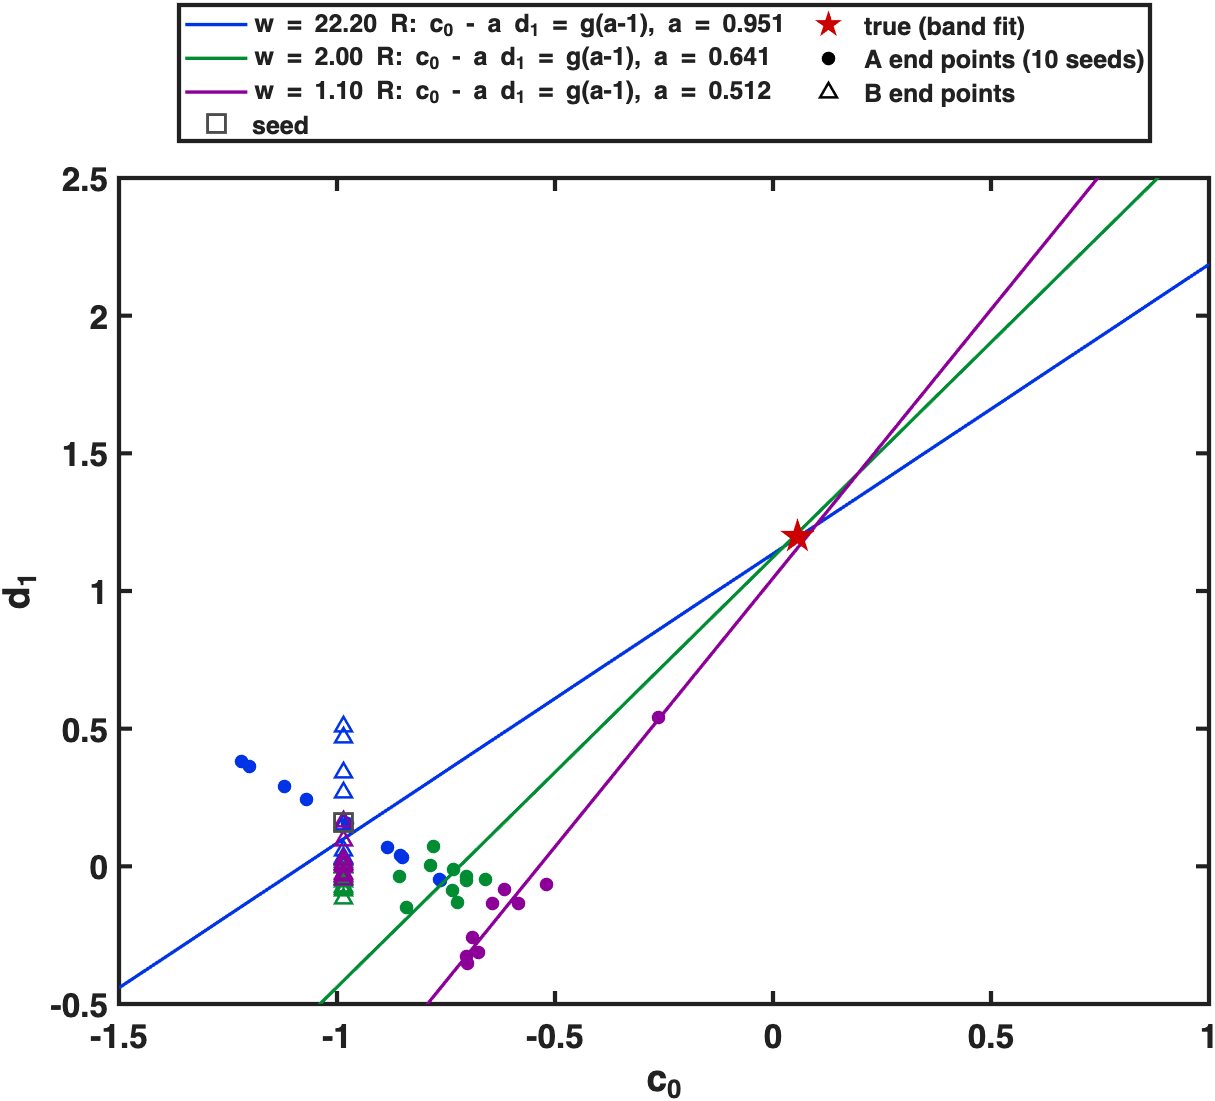
\includegraphics[width=\textwidth]{figures/fixed11_cell_cd.png}

\begin{landscape}
\vspace*{\fill}
\noindent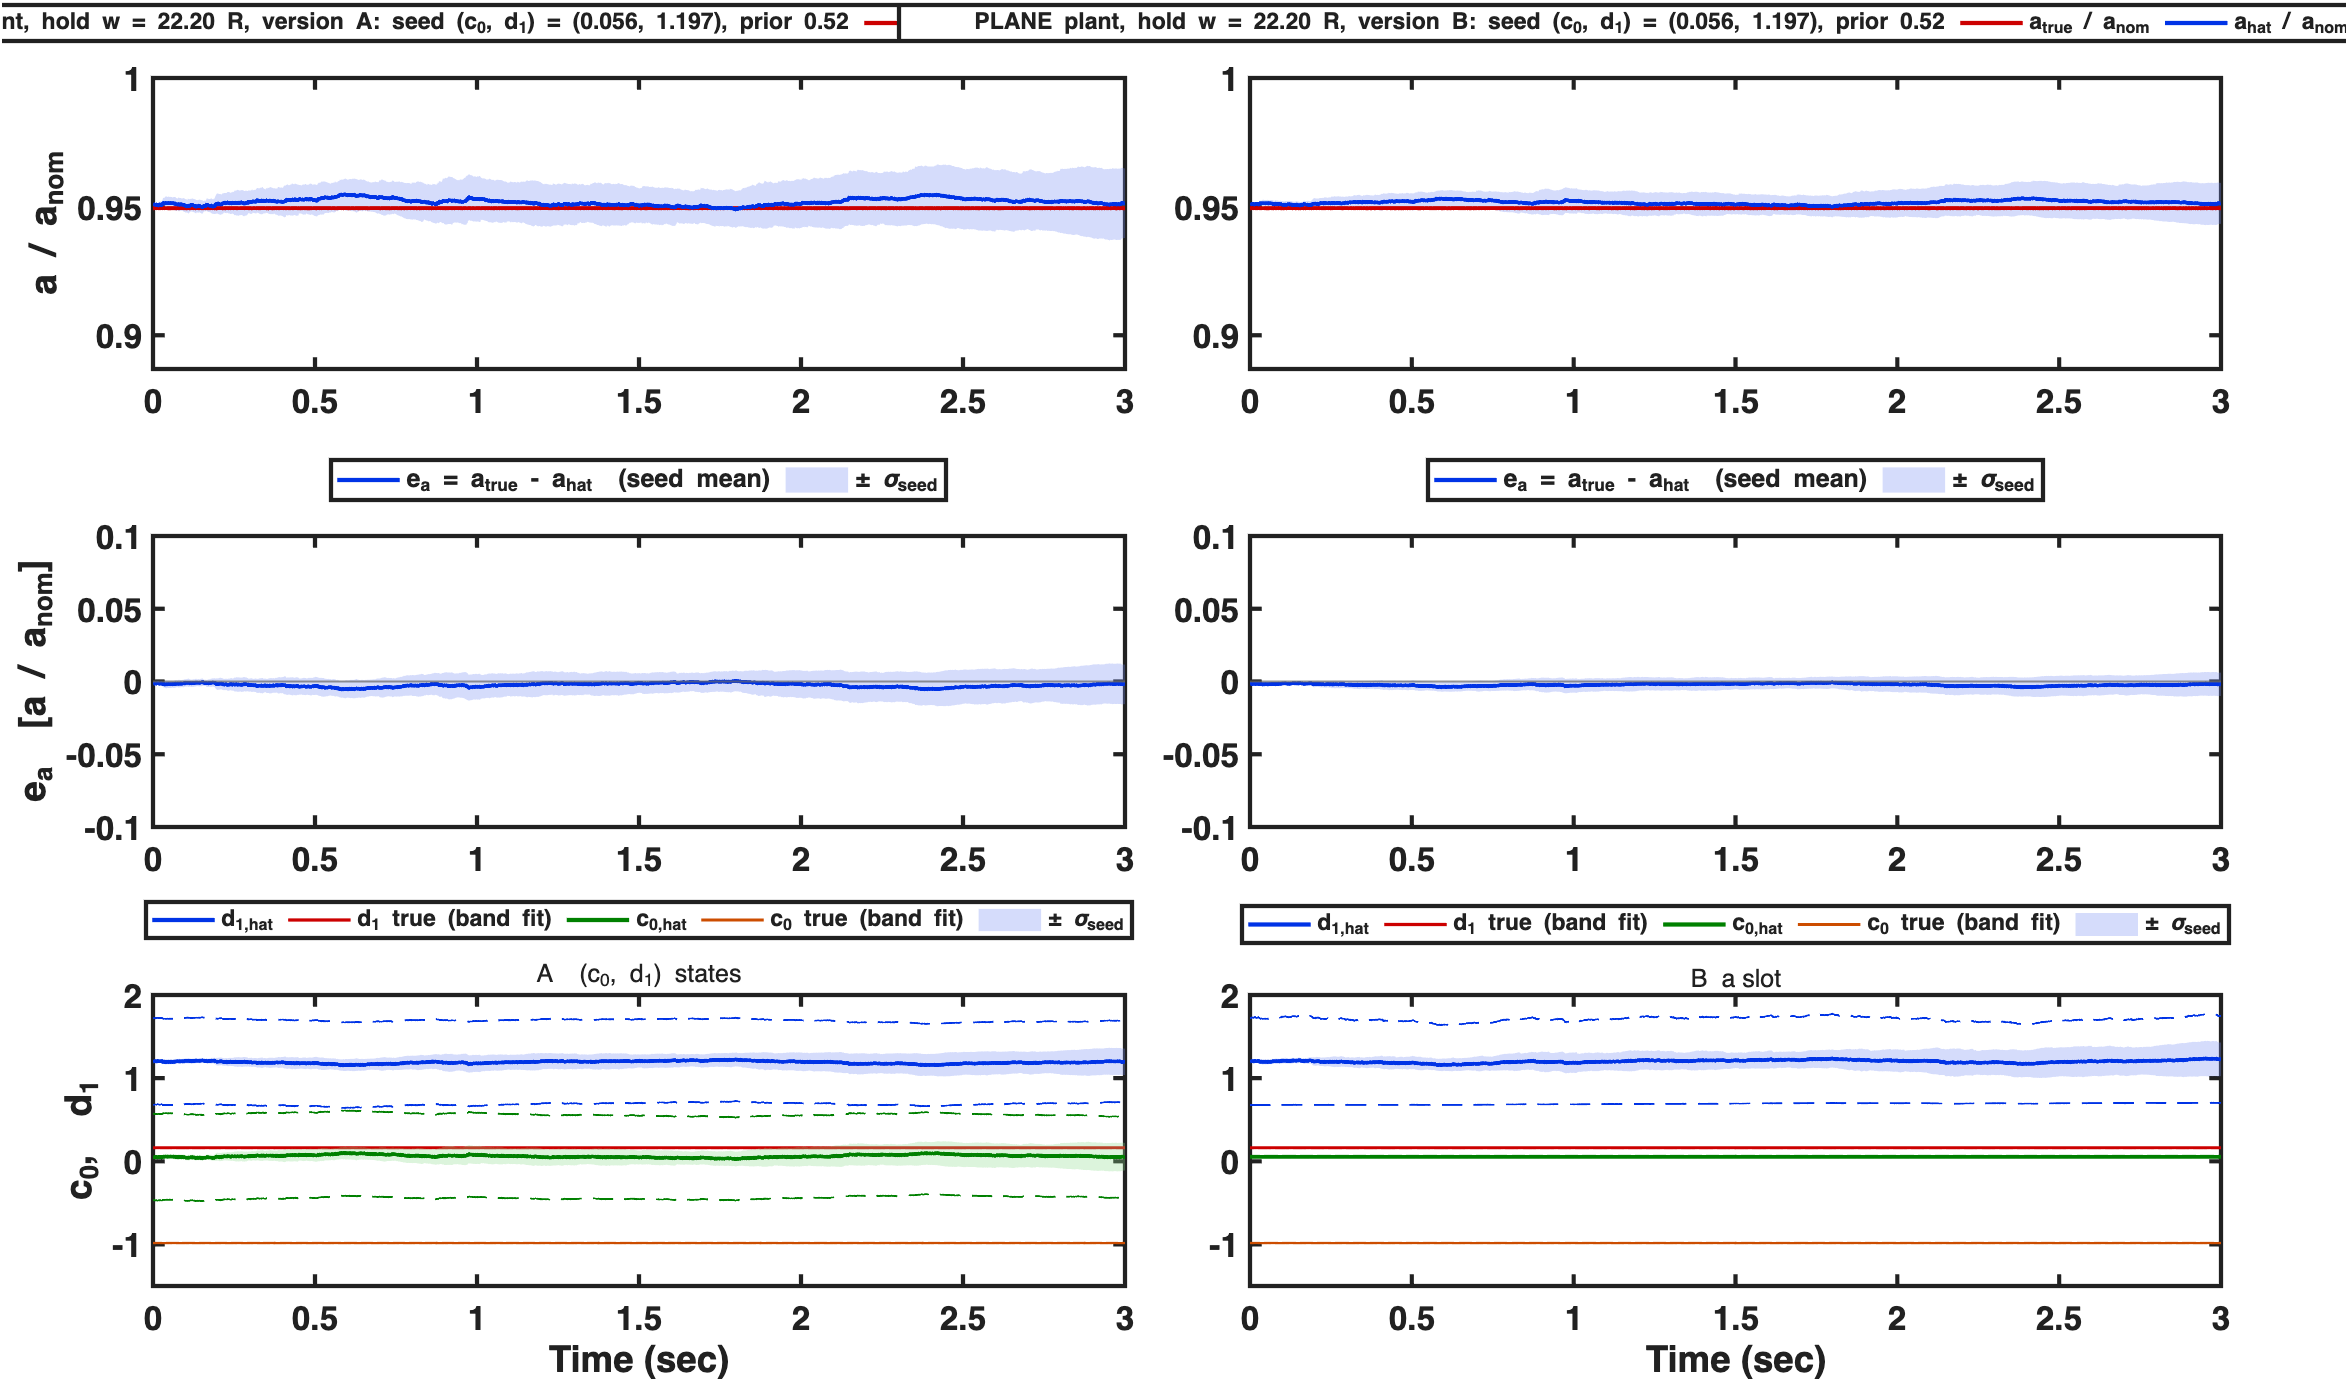
\includegraphics[width=\linewidth]{figures/fixed11_plane_h22p20.png}
\vspace*{\fill}
\end{landscape}

\begin{landscape}
\vspace*{\fill}
\noindent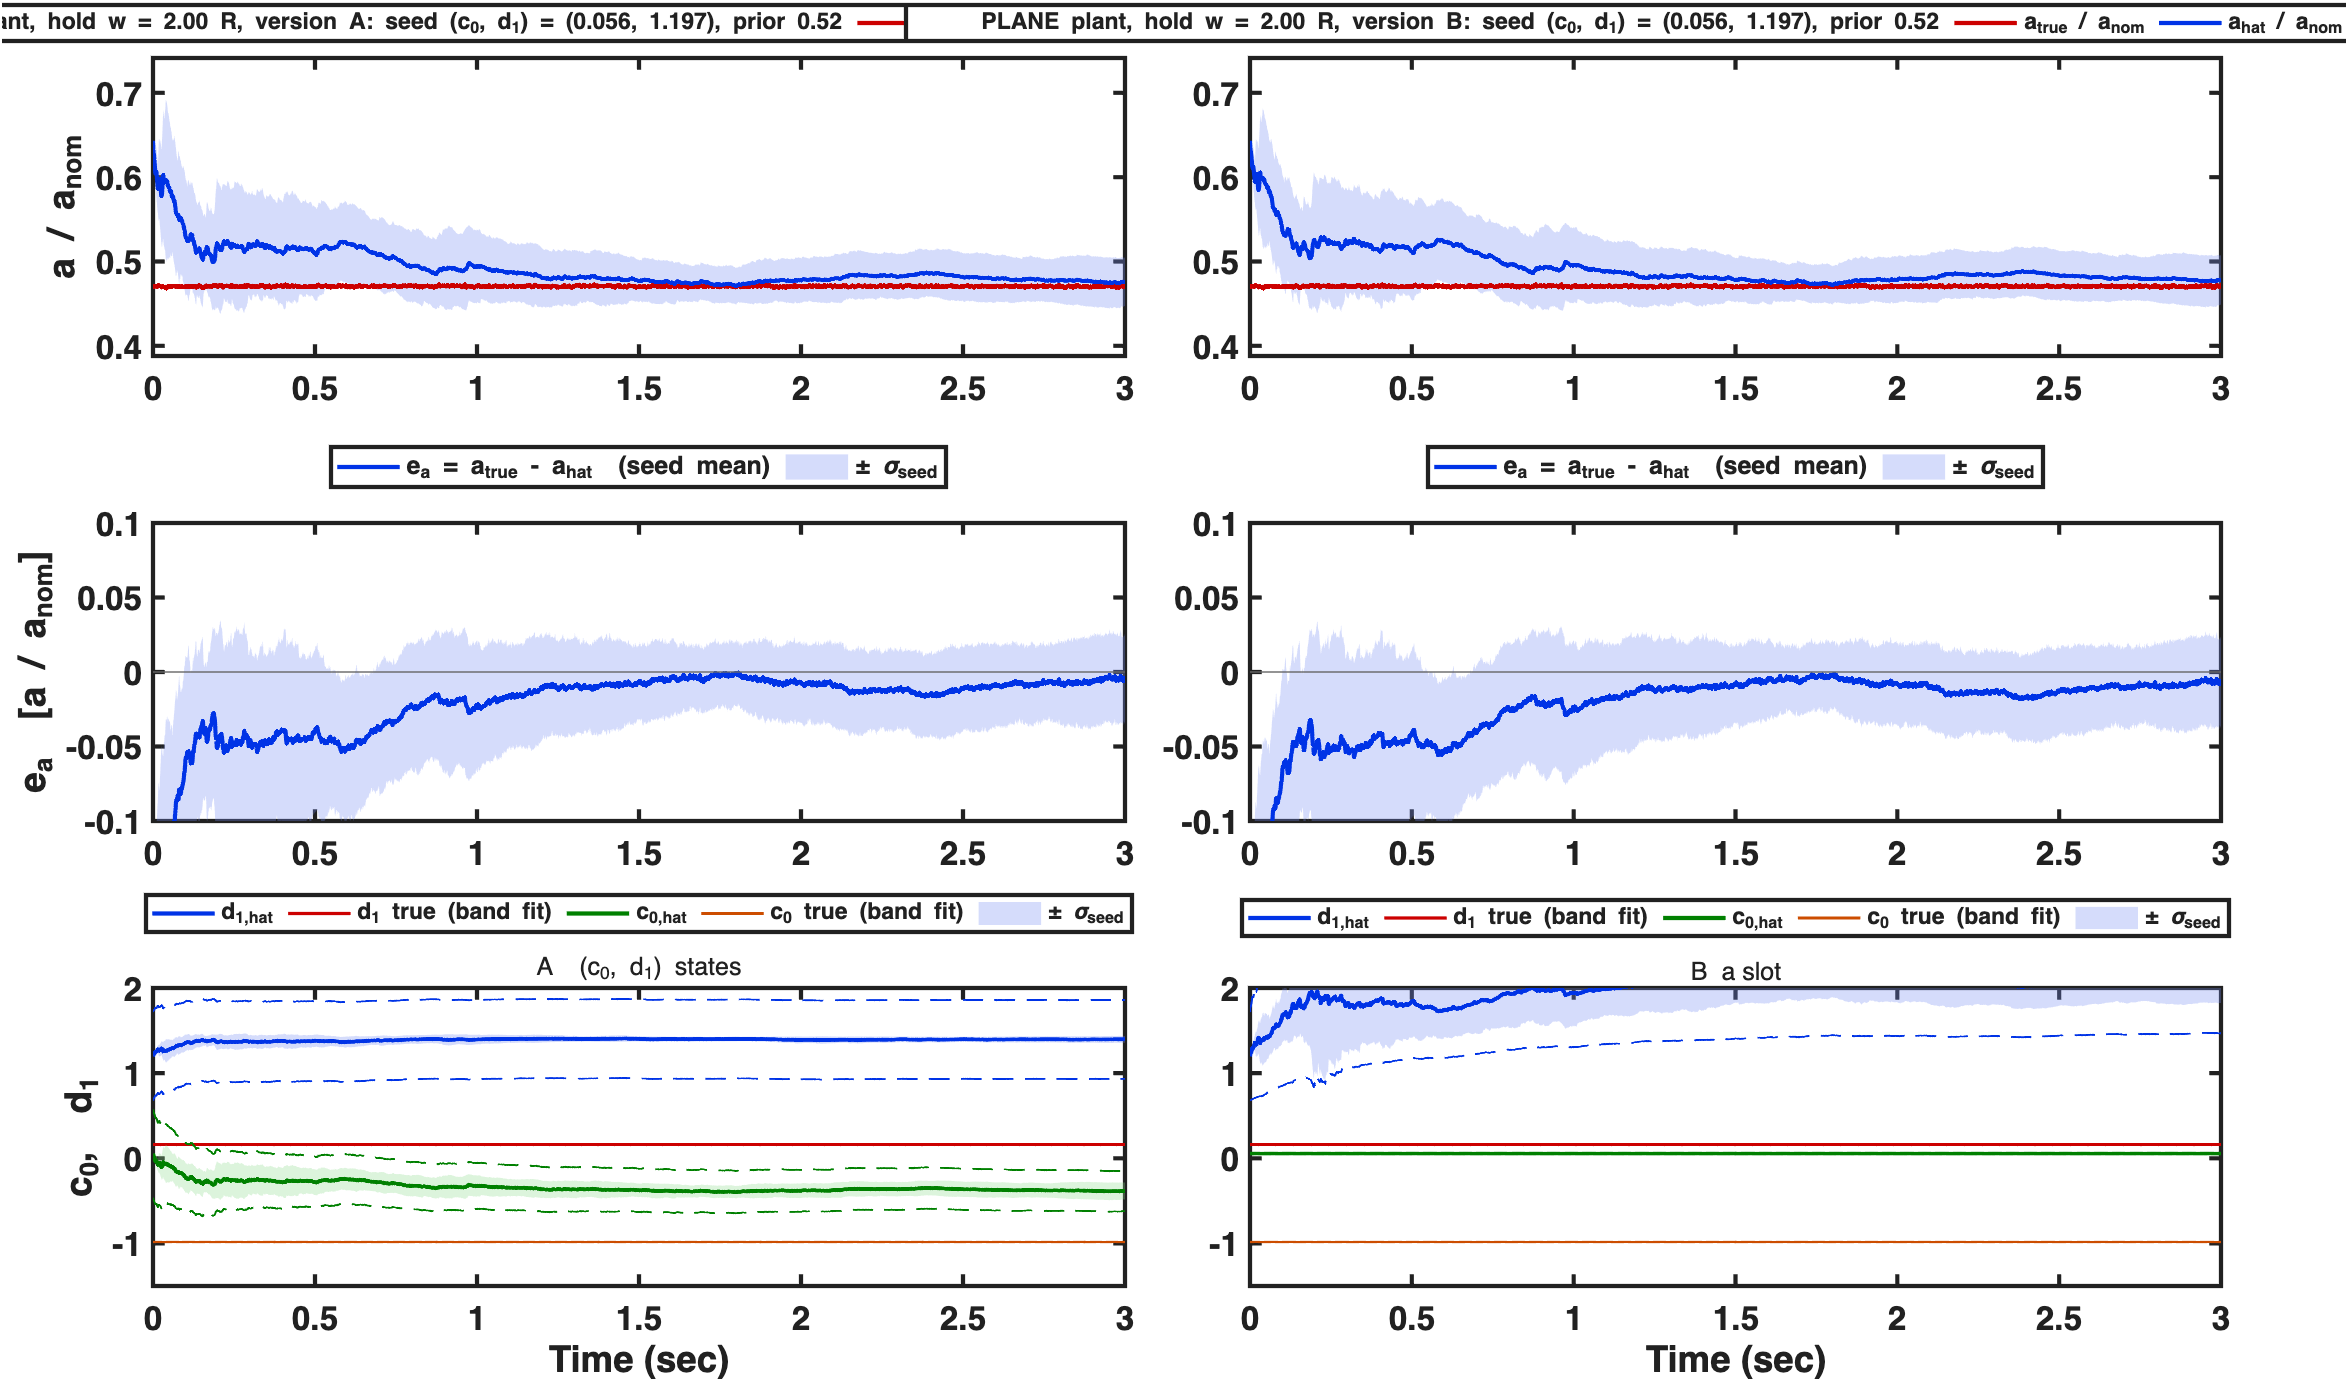
\includegraphics[width=\linewidth]{figures/fixed11_plane_h2p00.png}
\vspace*{\fill}
\end{landscape}

\begin{landscape}
\vspace*{\fill}
\noindent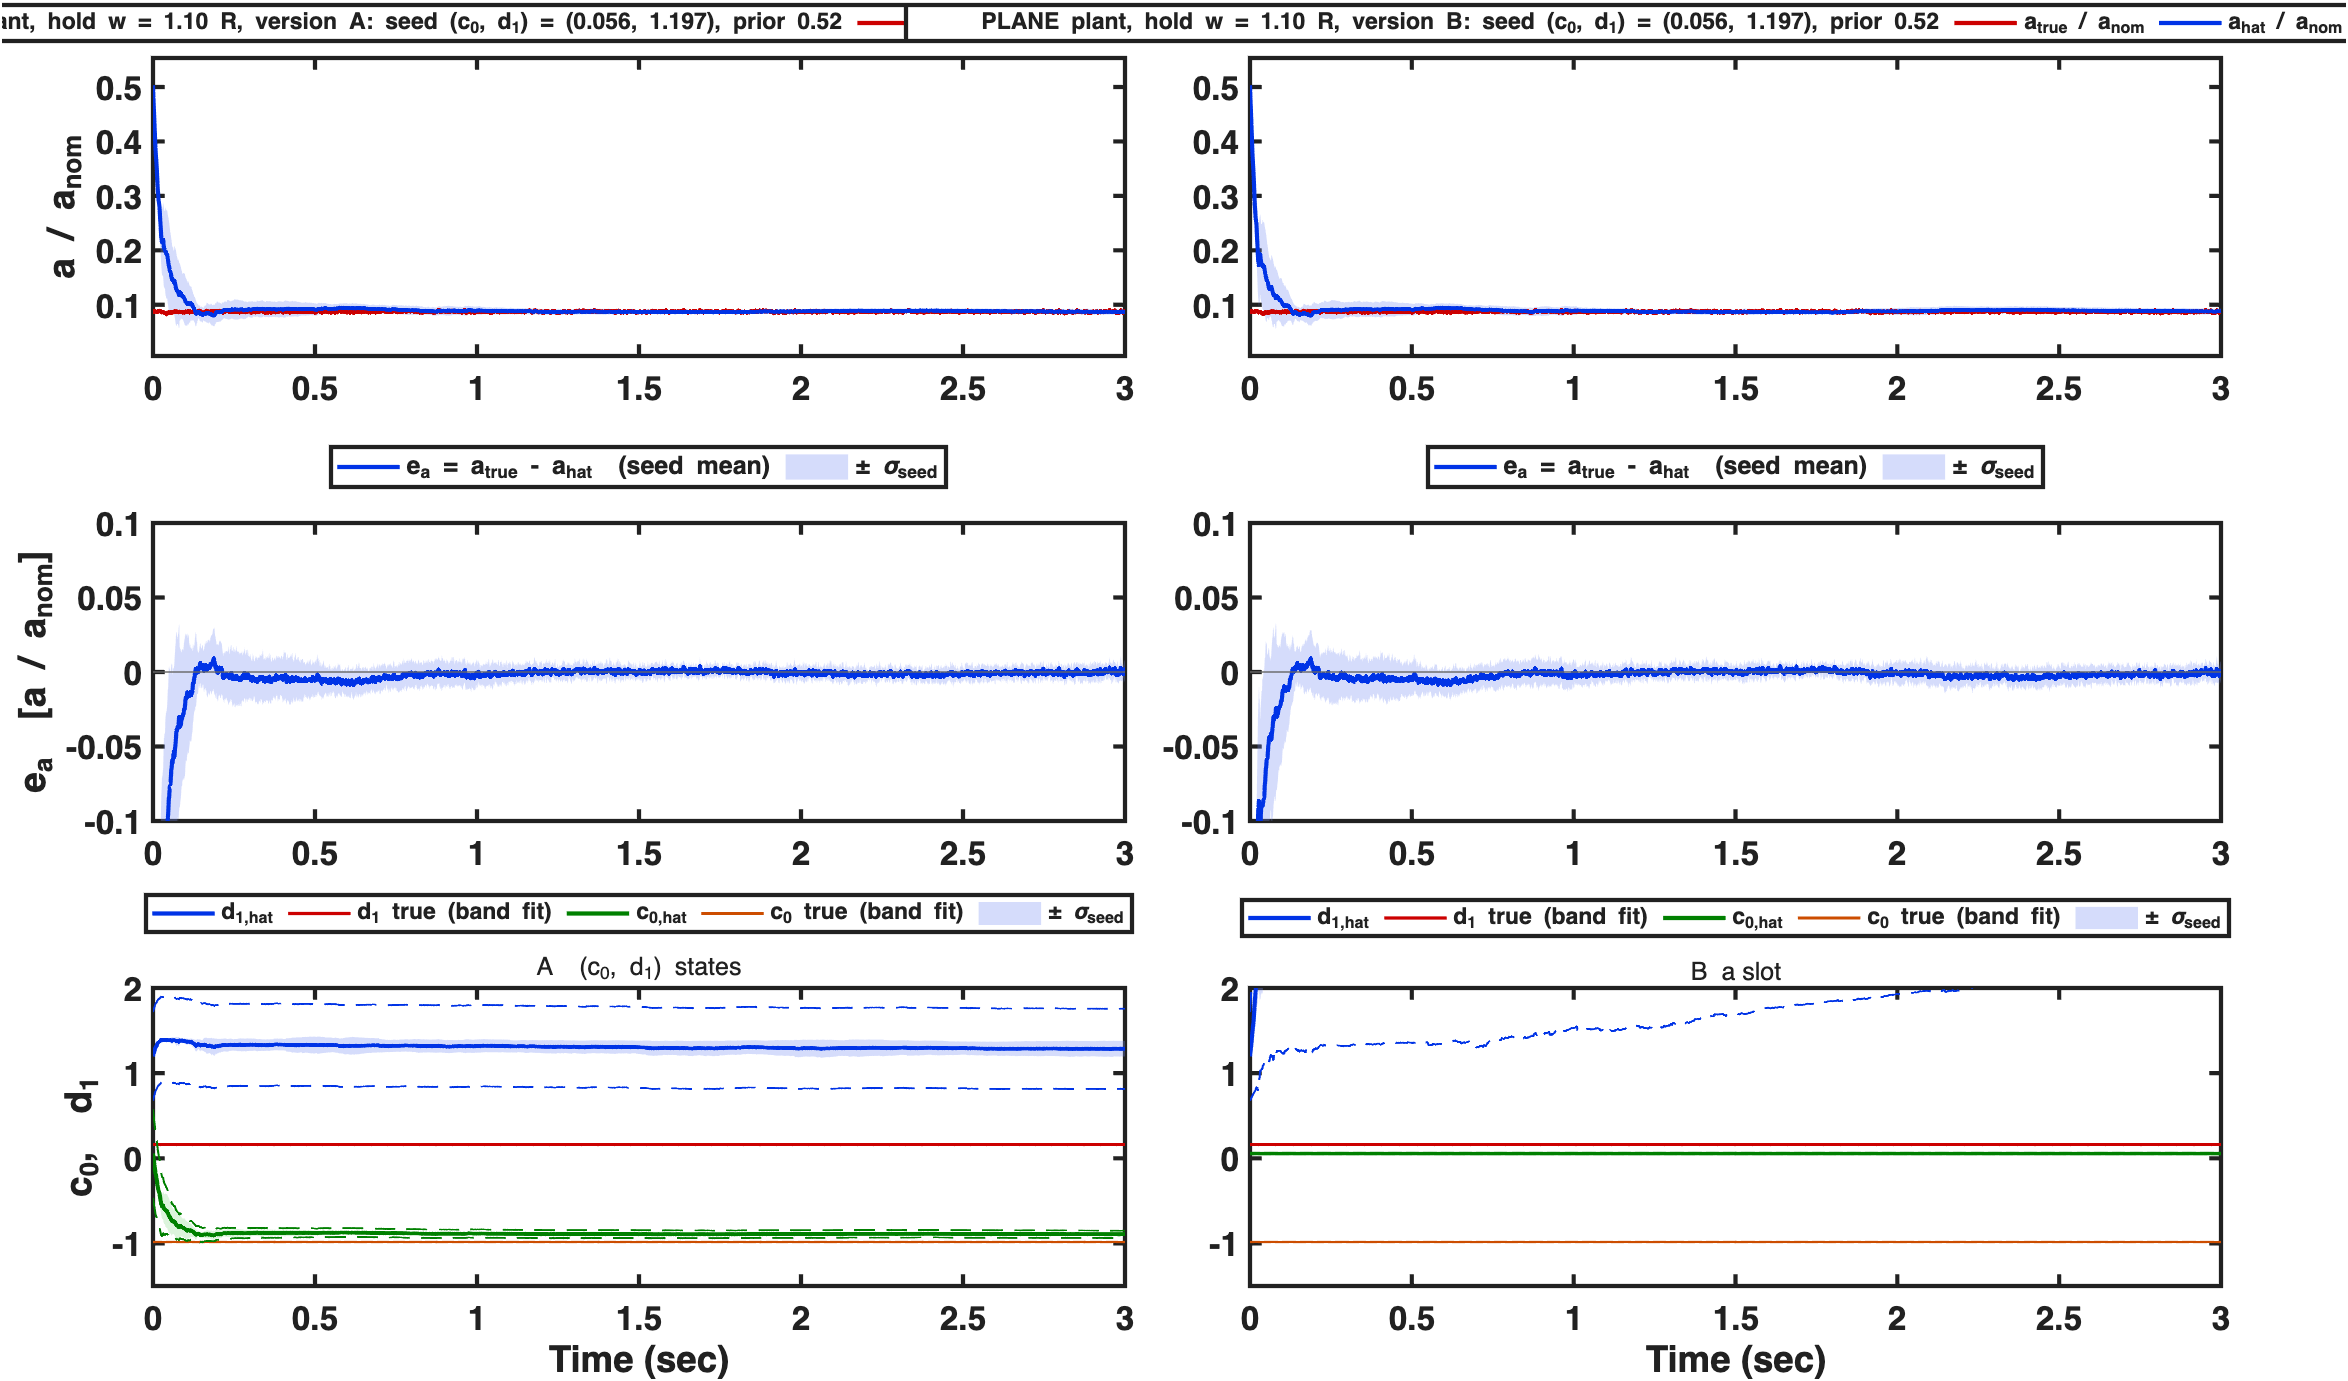
\includegraphics[width=\linewidth]{figures/fixed11_plane_h1p10.png}
\vspace*{\fill}
\end{landscape}

\clearpage
\noindent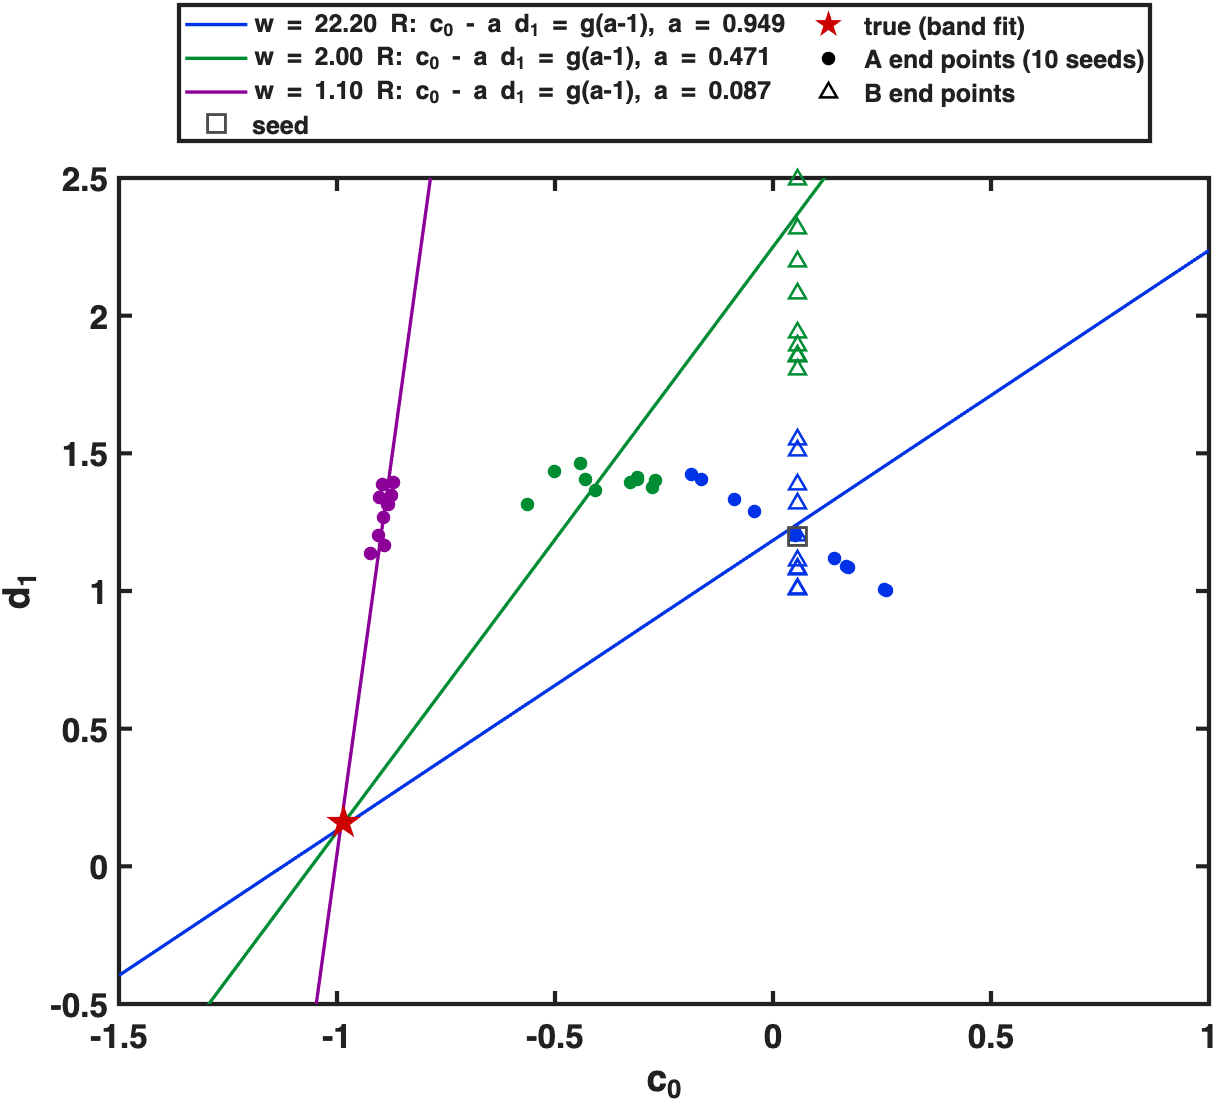
\includegraphics[width=\textwidth]{figures/fixed11_plane_cd.png}

\end{document}
